\documentclass{article}

% if you need to pass options to natbib, use, e.g.:
\PassOptionsToPackage{numbers,compress}{natbib}
% before loading main

% ready for submission
\usepackage{main}

% to compile a preprint version, e.g., for submission to arXiv:
% \usepackage[preprint]{main}

% to compile a camera-ready version:
% \usepackage[final]{main}

% to avoid loading the natbib package:
% \usepackage[nonatbib]{main}

\usepackage[utf8]{inputenc}
\usepackage[T1]{fontenc}
\usepackage[hypertexnames=false]{hyperref}
\hypersetup{hidelinks}
\usepackage{url}
\usepackage{xurl}
\usepackage{booktabs}
\usepackage{amsfonts}
\usepackage{nicefrac}
\usepackage{microtype}
\usepackage[table]{xcolor}
\usepackage{tabularx}
\usepackage{float}
\usepackage{graphicx}
\usepackage{listings}
\usepackage[all]{hypcap}
\usepackage{algorithm}
\usepackage{algorithmic}
\usepackage{amsmath}
\usepackage{amsthm}
\newtheorem{theorem}{Theorem}
\newtheorem{definition}{Definition}

\Urlmuskip=0mu plus 2mu\relax
\pdfstringdefDisableCommands{\def\our{ATTS}\def\attsmm{ATTS-MM}\def\explore{explore}\def\integrate{integrate}}

\newcommand\our{\makebox{\textsc{ATTS}}}
\newcommand\attsmm{\makebox{\textsc{ATTS-MM}}}
\newcommand\explore{\texttt{explore}}
\newcommand\integrate{\texttt{integrate}}
\newcommand{\groupheader}[2]{\rowcolor{gray!20}\multicolumn{#1}{c}{\textit{#2}}\\}
\newcommand{\sidegraphic}[1]{\vspace{0pt}\includegraphics[width=\textwidth,trim=8 8 8 0,clip]{#1}}
\makeatletter
\newcommand{\captionof}[1]{\def\@captype{#1}\caption}
\makeatother

\title{ATTS: Agentic Test-Time Scaling via Adaptive Exploration}
\author{
  Peijia Qin \\
  University of California, San Diego \\
  \texttt{pqin@ucsd.edu}
}

\begin{document}

\maketitle

\begin{abstract}
Test-time scaling has become a key lever for improving large language model reasoning, but existing approaches rely on rigid heuristic allocation or explicit search over intermediate reasoning steps. We introduce \our{}, a delegated sequential test-time scaling framework in which a lightweight orchestrator adaptively controls a pool of candidate solutions through a single action: \explore{}, which launches a fresh, independent solver. The orchestrator decides when to stop exploring and directly synthesizes the final answer from the accumulated evidence. The framework defines an extensible action space over solver dispatch decisions; we instantiate it with a single parameterless \explore{} tool and show that even this minimal configuration achieves strong results. We evaluate \our{} on six benchmarks spanning mathematical reasoning, scientific question answering, code generation, and multimodal reasoning. By stopping early when evidence converges, \our{} achieves competitive or superior accuracy with substantially fewer API calls than fixed-budget alternatives: 80.81\% on GPQA-Diamond, 82.29\% on LiveCodeBench, 56.00\% on HLE-Verified, and 23.20\% on BabyVision. An ablation (\our{} (+ Integrator)) replacing the orchestrator's direct synthesis with a separate integrator call degrades or fails to improve accuracy on three of four benchmarks, indicating that stateful evidence accumulation during exploration is critical to the method's effectiveness.
\end{abstract}

\section{Introduction}

Scaling inference-time compute improves large language model reasoning, but how to allocate that compute remains an open problem. No single strategy---sequential, parallel, or hybrid---is uniformly optimal across problems of varying difficulty \citep{snell_test_time_scaling_paper}, and naive scaling can saturate or even degrade accuracy through poor coverage and reward hacking \citep{best_of_n_optimality_paper}. The central question is not \emph{whether} to scale, but \emph{how} to allocate adaptively: reacting to evidence as it appears, and stopping when further exploration cannot justify its cost.

Existing approaches answer this question with either open-loop heuristics or explicit micro-level search. Predictive routing methods such as DiffAdapt use lightweight difficulty estimates to select an inference regime before generation begins, but these decisions cannot react to evidence that appears during reasoning \citep{diffadapt_paper}. At the other extreme, Tree of Thoughts and process-reward frameworks such as Math-Shepherd perform closed-loop adaptation through explicit tree expansion and step-level verification \citep{tree_of_thoughts_paper,math_shepherd_paper}. Recent agentic test-time scaling methods add further variants, but many still rely on statistical control rules such as vote entropy or confidence-triggered halting \citep{catts_webagents_paper,tumix_paper,general_agentbench_tts_paper}. An underexplored alternative is to delegate compute allocation entirely to an LLM orchestrator that makes sequential explore-or-stop decisions based on its assessment of accumulated evidence, without requiring explicit search trees or statistical stopping criteria.

We introduce \our{}, a \textbf{delegated sequential} test-time scaling framework that separates \emph{control} from \emph{solution generation}. A lightweight orchestrator manages a growing pool of candidate solutions through a single tool, \explore{}, which dispatches a fresh, independent solver on the original problem. When the orchestrator judges the accumulated evidence to be sufficient, it stops exploring and synthesizes the final answer directly. \our{} treats compute allocation as closed-loop decision-making over an \emph{extensible action space}: each \explore{} call can in principle specify which solver to invoke, at what reasoning effort, and with what decomposition strategy. We evaluate the simplest instantiation---a single parameterless tool whose only decision is when to stop---and show that even this minimal agent achieves competitive accuracy at substantially lower cost. \attsmm{}, a multi-model extension that adds model selection to the action space, yields further gains, supporting the principle that the orchestrator's value scales with the richness of its decision space.

We evaluate \our{} across four benchmarks spanning scientific question answering, code generation, and multimodal reasoning: HLE-Verified \citep{hle_verified_paper}, LiveCodeBench \citep{livecodebench_paper}, BabyVision \citep{babyvision_paper}, and GPQA-Diamond \citep{gpqa_paper}. Because the orchestrator is benchmark-agnostic, the same policy transfers across text-only and image-conditioned tasks.

Our contributions are as follows:
\begin{enumerate}\setlength{\itemsep}{1pt}\setlength{\parskip}{0pt}
    \item We introduce \our{}, a delegated sequential test-time scaling framework in which a lightweight orchestrator adaptively controls a pool of independent solvers through a single action (\explore{}), deciding when to stop based on accumulated evidence.
    \item We evaluate \our{} on six diverse benchmarks and show that it achieves competitive or superior accuracy to fixed-budget baselines while using substantially fewer API calls---80.81\% on GPQA-Diamond, 82.29\% on LiveCodeBench, and 56.00\% on HLE-Verified.
    \item Through ablations we show that the orchestrator's stateful evidence accumulation is critical: replacing direct synthesis with a separate integrator degrades accuracy on three of four benchmarks, and the framework generalizes across model families and action-space configurations.
\end{enumerate}

\section{Related Work}
\label{sec:related-work-conceptually}

\paragraph{Test-Time Scaling.} Inference-time compute for LLMs is commonly organized along three axes \citep{snell_test_time_scaling_paper}. \emph{Sequential scaling} increases reasoning depth within a single trajectory, including self-correction \citep{self_refine_paper}, budget-controlled decoding \citep{s1_budget_forcing_paper}, and long-thinking models that internalize extended chains of thought via reinforcement learning \citep{deepseek_r1_paper}. A critical negative result is that LLMs cannot self-correct reasoning through prompting alone \citep{cannot_self_correct_paper}, motivating architectures that separate evaluation from solution generation. \emph{Parallel scaling} increases reasoning width by sampling multiple independent candidates and aggregating them. Self-consistency marginalizes over diverse reasoning paths \citep{self_consistency_paper}; coverage scales log-linearly with the sample count \citep{large_language_monkeys_paper}; and Universal Self-Consistency uses the LLM itself to select among candidates for free-form tasks \citep{universal_self_consistency_paper}. Learned reward models and verifiers improve selection beyond majority voting \citep{snell_test_time_scaling_paper,skywork_reward_v2_paper,rasc_paper,visualprm_paper}, and Multi-Sequence Verifiers jointly process the entire candidate pool rather than scoring each independently \citep{msv_paper}. Theoretical analysis shows that naive parallel scaling is not uniformly beneficial: overly aggressive sampling can degrade accuracy through reward hacking \citep{best_of_n_optimality_paper,limiting_confidence_paper}. \emph{Hybrid search} combines depth and width by expanding and pruning partial trajectories via tree search \citep{tree_of_thoughts_paper}, Monte Carlo Tree Search with preference learning \citep{mcts_reasoning_paper}, step-level process reward models \citep{math_shepherd_paper}, or interleaved aggregation and refinement \citep{rsa_paper}. \our{} is neither a single-trajectory method nor a tree-search method: it delegates \emph{independent complete solves} to a separate explorer and manages the resulting candidate pool sequentially, occupying a distinct point in this design space.

\paragraph{Adaptive Compute Allocation.} A growing body of work addresses \emph{when} to stop sampling and \emph{how much} compute to allocate per problem. Statistical stopping criteria include Beta/Dirichlet confidence thresholds \citep{adaptive_consistency_paper}, the Sequential Probability Ratio Test \citep{consol_sprt_paper}, anytime-valid concentration bounds via e-processes \citep{certified_self_consistency_paper}, Bayesian optimal stopping with conjugate priors \citep{beacon_stopping_paper}, and optimal answer tracking showing that monitoring the top-3 answers suffices for asymptotic optimality \citep{optimal_bayesian_stopping_paper}. \citet{kalayci_optimal_stopping_bon} frame each generation as opening a box in Weitzman's Pandora's Box problem, deriving reservation-price stopping rules. On the learned side, \citet{damani_adaptive_allocation_paper} train a difficulty predictor to adapt the number of best-of-$k$ samples per query, and BEST-Route jointly selects which model and how many responses to sample \citep{best_route_paper}. These methods rely on either statistical criteria or learned scalar predictors. At the theoretical level, \citet{rational_metareasoning_llm_paper} operationalize rational metareasoning for LLMs at the \emph{token level}, training models with a VOC-derived reward that penalizes unnecessary reasoning steps within a single generation; they identify candidate-level agentic extension as an open direction. \our{} uses an LLM orchestrator that reads full reasoning traces---accessing richer information than answer frequencies or scalar scores---within a sequential closed loop where each observation informs the next action.

\paragraph{Agentic Orchestration.} Recent work studies both agentic test-time scaling and learned meta-level controllers. On the scaling side, CATTS allocates compute via vote-derived uncertainty \citep{catts_webagents_paper}, TUMIX coordinates parallel heterogeneous agents \citep{tumix_paper}, and General AgentBench benchmarks sequential and parallel scaling for open-ended agents \citep{general_agentbench_tts_paper}. On the meta-control side, \citet{adaptive_inference_time_paper} show that LLMs can predict mid-generation whether restarting will help; CoRefine attaches a lightweight controller that decides to halt, re-examine, or try a different approach \citep{corefine_paper}; Meta-Reasoner employs a contextual bandit over high-level strategies such as backtrack, restart, or switch approach \citep{meta_reasoner_paper}; AB-MCTS dynamically decides between expanding width and depth \citep{ab_mcts_paper,adaptive_ttc_bilal_paper}; and ORCH orchestrates multiple LLM analyses followed by a single merge \citep{orch_paper}. A parallel trend trains LLM orchestrators via reinforcement learning: Router-R1 uses GRPO for multi-round routing to external LLMs \citep{router_r1_paper}, xRouter learns cost-aware orchestration across 20+ models \citep{xrouter_paper}, and Search-R1 trains multi-turn search-interleaved reasoning \citep{search_r1_paper}. On multi-agent interaction, symmetric debate has been shown to induce a martingale over belief trajectories, providing no expected accuracy improvement beyond majority voting \citep{debate_or_vote_paper,can_llms_debate_paper}. \our{} differs from these approaches in one key respect: it dispatches \emph{fresh independent solvers} (not routing to different models or managing a single evolving trajectory), and only the orchestrator accumulates evidence---an asymmetric, delegated architecture with a single action type (\explore{}) whose value is assessed after each invocation.

\paragraph{Cost-Aware Agent Training.} A nascent line of work incorporates execution costs into agent objectives. CATP-LLM optimizes a performance-cost tradeoff for tool planning via cost-aware offline RL \citep{catp_llm_paper}. Calibrate-Then-Act formalizes the cost-uncertainty tradeoff for agent exploration, comparing the expected information value of an additional tool call against its cost \citep{calibrate_then_act_paper}. On reward engineering for tool use, ToolRL systematically studies reward type, scale, and granularity for GRPO-based training \citep{toolrl_paper}; StepTool assigns per-interaction rewards based on invocation success and task contribution \citep{steptool_paper}; and the Tool-call Reward Model enables step-level credit assignment in PPO/GRPO pipelines \citep{tool_call_rm_paper}. These works address planning, exploration, and reward design for general tool use. \our{} targets a more specific problem: \emph{candidate-level test-time scaling}, where the ``tool'' is an independent solver call and the meta-decision is a sequential explore-or-stop choice. To our knowledge, no prior work combines an LLM orchestrator that reads full candidate reasoning traces, sequential closed-loop stopping, and independently generated candidates within a unified framework for test-time compute allocation.

\section{Methodology}
\label{sec:methodology}

Test-time scaling is a resource allocation problem: given a budget of model calls, how should an agent decide what to compute next and when to stop? Drawing on the principle of \emph{rational metareasoning}~\citep{russell1991right,hay_selecting_computations}---that an agent should reason about whether additional computation justifies its cost---we design \our{} as a delegated sequential framework in which a lightweight orchestrator manages a growing pool of candidate solutions, decides when to stop exploring, and synthesizes the final answer from the accumulated evidence.

\subsection{The \our{} Loop}

The orchestrator repeatedly decides whether to call \explore{} or to stop and synthesize. It \emph{never} solves the problem itself.

\paragraph{Explore.} Each \explore{} call dispatches a fresh solver on the original problem \(x\). The solver works \emph{from scratch}---it does not see or continue previous candidates---and returns a structured candidate \(c_t = (\text{answer}, \text{reasoning}, \text{approach}, \text{confidence})\) that is appended to \(\mathcal{C}_t\). By construction, each explorer receives only the problem statement, guaranteeing that explore results are \emph{conditionally independent} given the problem. This independence means the orchestrator can assess the marginal contribution of each additional explore in isolation, without modeling interactions between future computations.

\paragraph{Stopping.} The orchestrator can stop at any point before the exploration budget \(T\) is exhausted. The stopping decision is made by the orchestrator model itself based on its assessment of the candidate pool. The prompt encodes principles for this judgment: genuine convergence means independent solvers arriving at the same answer through different methods, repeated failures indicate the problem exceeds solver capability, and each additional explore call has a cost that must be justified by expected information gain. This judgment reflects the same cost-benefit tradeoff formalized by the \emph{value-of-computation} criterion~\citep{hay_selecting_computations}: additional exploration is warranted only when the expected information gain justifies the cost.

\paragraph{Synthesis.} When the orchestrator stops, it synthesizes the final answer directly from \(\mathcal{C}_t\). Because it has observed the full multi-turn history---each candidate's arrival, its reasoning, and its own deliberation about whether to continue---it has richer context than a separate aggregator that only sees the final pool.

\begin{algorithm}[t]
\caption{\our{}: Adaptive Test-Time Scaling}
\label{alg:atts}
\begin{algorithmic}[1]
\REQUIRE Problem $x$, exploration budget $T$, orchestrator LLM $\mathcal{O}$, solver LLM $\mathcal{S}$
\ENSURE Final answer $y$
\STATE $\mathcal{C} \leftarrow \emptyset$ \COMMENT{candidate pool}
\FOR{$t = 1$ \TO $T$}
    \STATE \textit{action} $\leftarrow \mathcal{O}(x, \mathcal{C})$ \COMMENT{decide: explore or stop}
    \IF{\textit{action} = \texttt{stop}}
        \STATE \textbf{break}
    \ENDIF
    \STATE $c_t \leftarrow \mathcal{S}(x)$ \COMMENT{fresh, independent solve}
    \STATE $\mathcal{C} \leftarrow \mathcal{C} \cup \{c_t\}$
\ENDFOR
\STATE $y \leftarrow \mathcal{O}(x, \mathcal{C})$ \COMMENT{synthesize final answer}
\RETURN $y$
\end{algorithmic}
\end{algorithm}

Algorithm~\ref{alg:atts} summarizes the procedure. The control logic is benchmark-agnostic: only the explorer prompt and answer schema change across tasks. The orchestrator prompt encodes its decision logic as declarative principles (e.g.\ ``a single candidate does not constitute sufficient evidence'') rather than prescriptive rules, paired with worked examples that demonstrate how these principles apply in concrete scenarios. Appendix~\ref{app:implementation-details} gives the full implementation details including representative prompts.

\subsection{Extensible Action Space}

The value of the framework scales with the richness of the orchestrator's action space. In the simplest instantiation, the only action is ``explore once more with the same model,'' and the orchestrator can only decide \emph{when} to stop. With heterogeneous computation types, it also decides \emph{what} to compute---selecting among different effort levels, solver models, or time budgets based on the current evidence. Each extension adds degrees of freedom for adapting to problem difficulty without changing the underlying loop.

This yields a concrete design principle: \our{}'s architecture is not a fixed pipeline but a framework for adaptively selecting what to compute at test time, in the spirit of \citet{hay_selecting_computations}. The experiments in this paper evaluate the simplest instantiation, \our{} (single model, uniform effort), alongside \attsmm{}, a multi-model extension with configurable exploration effort (\S\ref{sec:experiments}).

\subsection{Multi-Model Extension (\attsmm{})}

We define \attsmm{} by extending \our{} with model selection in the orchestrator's decision space. The orchestrator (Claude Sonnet 4.6) dispatches explores to a pool of three models---Haiku (cheapest), Sonnet (mid-range), and Opus (strongest)---each with a per-question budget limit. Model profiles inform dispatch decisions: the orchestrator starts with cheaper models, escalates on disagreement or repeated failure, and treats cross-model agreement as stronger evidence than same-model convergence. This enables cost-aware exploration strategies where easy problems are solved entirely with cheap models while hard problems automatically escalate to more capable solvers. An \emph{exploration effort} parameter controls the exploration policy: Low effort instructs the orchestrator to stop as soon as any two candidates converge, Medium effort requires at least three explores across at least two different models before the orchestrator's stopping judgment takes effect, and High effort requires at least five explores using all three models.

\section{Experiments}
\label{sec:experiments}

We evaluate on four benchmarks: HLE-Verified \citep{hle_verified_paper}, LiveCodeBench \citep{livecodebench_paper}, BabyVision \citep{babyvision_paper}, and GPQA-Diamond \citep{gpqa_paper}, which collectively span scientific question answering, code generation, and multimodal reasoning. Appendix~\ref{app:benchmark-details} collects the full official task definitions, grading rules, source repositories, and leaderboard alignment notes for all benchmarks.

\subsection{Experimental Setup}

% =============================================================================
% NAMING REFERENCE -- ATTS method variants (do not edit lightly).
% Two main methods (always reported with bare names):
%
%   Axis              | ATTS                       | ATTS-MM
%   ------------------|----------------------------|--------------------------
%   Solver pool       | Sonnet 4.6 (single)        | {Haiku, Sonnet, Opus}
%   Effort            | --                         | Medium
%   Synthesis         | orchestrator-direct        | orchestrator-direct
%   Orch thinking     | enabled                    | enabled
%   Orchestrator      | Sonnet 4.6                 | Sonnet 4.6
%   Budget T          | 8                          | 16 (Haiku 8, Sonnet 8, Opus 4)
%
% Ablation variants (deviate on one axis only; name pattern: BASE (deviation)):
%   ATTS (+ Integrator)     -- adds separate \integrate{} step (Tab 2)
%   ATTS (no thinking)      -- disables extended thinking (Tab 4)
%   ATTS (Haiku orch)       -- swaps orchestrator only (App B Tab 6)
%   ATTS (Opus orch)        -- swaps orchestrator only (App B Tab 6)
%   ATTS w/ GPT-5.2 backbone (Tab 3) -- backbone family swap, all roles
%   ATTS-MM (Low) / ATTS-MM (High)   -- effort sweep (App B Tab 5)
%
% Forbidden phrasings (do NOT reintroduce -- collapsed during cleanup):
%   "ATTS (Ours)", "ATTS Multi-model Med", "ATTS Multi Med",
%   "the multi-model variant", "single-model ATTS configuration",
%   "default ATTS architecture", "Default (no integrator)",
%   "Thinking disabled" as standalone label, "Sonnet orchestrator" as suffix.
% =============================================================================

The experiments below evaluate two configurations of our framework, treated as the two methods we report. \our{} is the single-model configuration: Claude Sonnet 4.6 (\texttt{claude-sonnet-4-6}) serves as both orchestrator and explorer, the orchestrator synthesizes the final answer directly (no separate integrator), extended thinking is enabled, and the exploration budget is $T{=}8$ \explore{} calls per question. \attsmm{} is the multi-model configuration: the orchestrator (still Sonnet 4.6) dispatches to a pool of three explorers \{Haiku, Sonnet, Opus\} at Medium exploration effort, with budget $T{=}16$ (per-model limits: Haiku~8, Sonnet~8, Opus~4). Unless otherwise noted, all baselines and ablation variants share the same backbone (Sonnet 4.6), default sampling parameters (no explicit temperature or top-$p$ override), extended thinking budget of 32{,}000 tokens, and the API's default reasoning effort. Claude Haiku, Sonnet, and Opus are three capability tiers in the Claude model family, ordered from smallest/cheapest to largest/most capable.

We compare against seven baselines, all sharing the same backbone model and answer interface so that only the inference-time strategy differs (full details in Appendix~\ref{app:implementation-details}): Pass@1 (single rollout), Majority Voting ($N{=}8$ independent candidates, most-frequent answer; reported only on benchmarks where direct answer aggregation is well-defined), Self-Refine~\citep{self_refine_paper} (iterative feedback-revision on a single draft), Socratic Self-Refine~\citep{socratic_self_refine_paper} (Self-Refine with the feedback step replaced by Socratic-style probing questions before revision), Budget Forcing~\citep{s1_budget_forcing_paper} ($N$ sequential rounds with forced continuation via ``Wait''), reward-model reranking using Skywork-Reward-V2~\citep{skywork_reward_v2_paper,skywork_reward_v2_hf} for text benchmarks or VisualPRM~\citep{visualprm_paper,visualprm_hf} for multimodal benchmarks, and LLM Selection ($N{=}8$), which feeds all pre-cached candidates to the backbone model in a single call and asks it to analyze, compare, and synthesize a final answer. LLM Selection isolates the contribution of LLM-based aggregation from adaptive sequential exploration.

For \our{}, the controller issues up to the exploration budget of \explore{} calls before stopping and synthesizing the final answer directly, as described in Section~\ref{sec:methodology}. The comparison across all rows isolates differences in test-time inference strategy rather than differences in training data, parameter count, or post-training recipe.

\paragraph{Cost accounting.} All costs reported as \$/q reflect API token charges only, computed from per-model pricing and recorded token usage. For \our{}, this includes orchestrator tokens, explorer tokens, and (when applicable) integrator tokens. For reward-model reranking, the reported cost covers the $N{=}8$ candidate generation calls; the reward model itself runs locally and incurs no API cost but does require GPU compute not reflected in the dollar figure. Grading costs (LLM judge calls for HLE and BabyVision) are excluded from all rows. In all tables, \textbf{bold} marks the best accuracy per group and the lowest \$/q among test-time scaling methods.

\paragraph{Run-to-run stability.} To assess variance, we run \our{} five times on GPQA-Diamond with different random seeds (varying the order of questions and orchestrator sampling). The results are highly stable: $80.20\% \pm 0.55\%$ (range: $79.8\%$--$80.8\%$, $\sigma = 0.55$), with cost $\$0.32 \pm \$0.01$/q. The standard deviation of 0.55 percentage points corresponds to a difference of approximately two questions across runs, indicating that the orchestrator's stopping and synthesis decisions are robust to sampling stochasticity. All other results in the paper are single-run evaluations; the GPQA stability analysis suggests that the reported numbers are representative.

\begin{table}[t!]
\centering
\caption{Main results on four benchmarks. Top left: HLE-Verified (Accuracy). Top right: LiveCodeBench (Pass@1, overall and by difficulty). Bottom left: GPQA-Diamond (Accuracy). Bottom right: BabyVision (Avg@3, overall and by task family). Each subtable shows zero-shot model references (upper) and test-time scaling methods (lower). \textbf{Bold} marks the best per group; lowest \$/q among test-time methods is also bolded.}
\label{tab:main-results}
\scriptsize
\setlength{\tabcolsep}{2pt}
\begin{minipage}[t]{0.38\textwidth}
\centering
\textit{(a) HLE-Verified}\\[3pt]
\begin{tabular}{l r r}
\toprule
 & Acc. (\%) & \$/q \\
\midrule
\groupheader{3}{Zero-Shot Models}
Gemini 3 Pro & 48.93 & -- \\
GPT-5.2-High & \textbf{52.48} & -- \\
Claude Opus 4.5 & 48.16 & -- \\
Grok 4.1 Fast Reasoning & 43.07 & -- \\
Claude Opus 4.6 & 50.16 & -- \\
DeepSeek-V3.2 & 47.45 & -- \\
Qwen3-Max-Thinking & 48.48 & -- \\
\midrule
\groupheader{3}{Test-Time Scaling Methods}
Pass@1 & 48.00 & 0.50 \\
Self-Refine & 53.00 & \textbf{0.41} \\
Socratic Self-Refine & 45.00 & 0.90 \\
Budget Forcing & 51.00 & 0.60 \\
% Corrected: 10 compaction-failed explores in hle/sonnet/gold cache zeroed (cost_usd -> 0).
% Skywork/LLM Selection read all 8 explores per question -> all 10 bad explores consumed -> -$79.40.
% Skywork: ($440.73-$79.40)/100 = $3.61. LLM Selection: ($449.95-$79.40)/100 = $3.71.
% ATTS (v3): 4 of 10 consumed -> -$31.68 -> ($190.47-$31.68)/100 = $1.59.
% Multi-model Med: 1 of 10 consumed -> -$8.63 -> ($162.80-$8.63)/100 = $1.54.
Skywork-Reward-V2 & 52.00 & 3.61 \\
LLM Selection ($N{=}8$) & \textbf{58.00} & 3.71 \\
\our{} & 56.00 & 1.59 \\
\attsmm{} & 57.00 & 1.54 \\
\bottomrule
\end{tabular}
\end{minipage}\hfill%
\begin{minipage}[t]{0.60\textwidth}
\centering
\textit{(b) LiveCodeBench}\\[3pt]
\begin{tabular}{l r r r r r}
\toprule
 & Pass@1 & Easy & Med. & Hard & \$/q \\
\midrule
\groupheader{6}{Zero-Shot Models}
O4-Mini (High) & \textbf{80.2} & \textbf{99.1} & \textbf{89.4} & \textbf{63.5} & -- \\
O3 (High) & 75.8 & \textbf{99.1} & 84.4 & 57.1 & -- \\
O4-Mini (Med.) & 74.2 & 98.2 & 86.5 & 52.7 & -- \\
Gemini-2.5-Pro & 73.6 & \textbf{99.1} & 87.2 & 50.2 & -- \\
DeepSeek-R1 & 73.1 & 98.7 & 85.2 & 50.7 & -- \\
\midrule
\groupheader{6}{Test-Time Scaling Methods}
Pass@1 & 77.14 & 95.35 & 88.46 & 60.00 & \textbf{0.24} \\
Self-Refine & 80.57 & \textbf{100.00} & 90.38 & 63.75 & 0.32 \\
Socratic Self-Refine & 82.29 & \textbf{100.00} & 90.38 & 67.50 & 0.60 \\
Budget Forcing & 80.00 & \textbf{100.00} & 88.46 & 63.75 & 0.50 \\
Skywork-Reward-V2 & 78.86 & \textbf{100.00} & 90.38 & 60.00 & 1.41 \\
LLM Selection ($N{=}8$) & 81.14 & \textbf{100.00} & 86.54 & 67.50 & 1.51 \\
\our{} & 82.29 & \textbf{100.00} & 90.38 & 67.50 & 0.53 \\
\attsmm{} & \textbf{85.63} & \textbf{100.00} & \textbf{92.31} & \textbf{73.42} & 0.69 \\
\bottomrule
\end{tabular}
\end{minipage}

\vspace{6pt}

\begin{minipage}[t]{0.38\textwidth}
\centering
\textit{(c) GPQA-Diamond}\\[3pt]
\begin{tabular}{l r r}
\toprule
 & Acc. (\%) & \$/q \\
\midrule
\groupheader{3}{Zero-Shot Models}
Gemini 3.1 Pro Preview & \textbf{94.1} & -- \\
GPT-5.4 (xhigh) & 92.0 & -- \\
GPT-5.3 Codex (xhigh) & 91.5 & -- \\
Gemini 3 Pro Preview (high) & 90.8 & -- \\
GPT-5.2 (xhigh) & 90.3 & -- \\
\midrule
\groupheader{3}{Test-Time Scaling Methods}
Pass@1 & 74.24 & \textbf{0.13} \\
Majority Voting & 73.74 & 0.90 \\
Self-Refine & 73.10 & 0.23 \\
Socratic Self-Refine & 74.24 & 0.56 \\
Budget Forcing & 77.16 & 0.42 \\
Skywork-Reward-V2 & 76.14 & 0.90 \\
LLM Selection ($N{=}8$) & 77.16 & 0.97 \\
\our{} & 80.81 & 0.34 \\
\attsmm{} & \textbf{81.82} & 0.39 \\
\bottomrule
\end{tabular}
\end{minipage}\hfill%
\begin{minipage}[t]{0.60\textwidth}
\centering
\textit{(d) BabyVision}\\[3pt]
\begin{tabular}{l r r r r r r}
\toprule
 & Overall & Fine-gr. & Tracking & Spatial & Pattern & \$/q \\
\midrule
Human & 94.1 & 92.3 & 94.6 & 94.7 & 97.8 & -- \\
\midrule
\groupheader{7}{Zero-Shot Models}
Gemini3-Pro-Preview & \textbf{49.7} & \textbf{46.2} & \textbf{43.4} & \textbf{53.7} & 53.9 & -- \\
GPT-5.2 & 34.4 & 27.3 & 34.9 & 35.2 & \textbf{54.9} & -- \\
Doubao-1.8 & 30.2 & 39.2 & 15.7 & 24.7 & 37.7 & -- \\
Qwen3-VL-Plus & 19.2 & 21.8 & 11.5 & 18.1 & 25.5 & -- \\
Grok-4 & 16.2 & 11.0 & 24.1 & 13.2 & 24.8 & -- \\
\midrule
\groupheader{7}{Test-Time Scaling Methods}
Pass@1 & 19.59 & 20.86 & 19.28 & 19.78 & 15.69 & \textbf{0.07} \\
Majority Voting & \textbf{23.20} & \textbf{23.93} & 21.69 & 23.08 & \textbf{23.53} & 0.50 \\
Self-Refine & 21.39 & 20.25 & 22.89 & 20.88 & \textbf{23.53} & 0.42 \\
Socratic Self-Refine & 21.13 & 18.40 & 25.30 & 20.88 & \textbf{23.53} & 0.58 \\
Budget Forcing & 21.91 & 20.86 & \textbf{28.92} & 21.98 & 13.73 & 0.52 \\
VisualPRM & 20.88 & 20.86 & 21.69 & 21.98 & 17.65 & 0.50 \\
LLM Selection ($N{=}8$) & \textbf{23.20} & 23.31 & 25.30 & 23.08 & 19.61 & 0.56 \\
\our{} & \textbf{23.20} & 22.09 & 24.10 & \textbf{26.37} & 19.61 & 0.27 \\
\attsmm{} & 22.42 & 22.09 & 27.71 & 21.98 & 15.69 & 0.43 \\
\bottomrule
\end{tabular}
\end{minipage}
\end{table}

\subsection{\our{} Achieves Competitive Accuracy at Lower Cost}

Table~\ref{tab:main-results} presents the main results across all four benchmarks. For each benchmark, the upper group reproduces published zero-shot references for context, and the lower group reports test-time scaling methods evaluated under our unified setup. Zero-shot references are cited from the respective benchmark papers and official leaderboards; they use different model configurations and are therefore not directly comparable to our test-time scaling rows. HLE-Verified zero-shot rows report Revised-subset Acc \citep{hle_verified_paper} while our rows evaluate a 100-sample Gold subset. LiveCodeBench references follow the public generation leaderboard \citep{livecodebench_paper}. BabyVision references are from \citet{babyvision_paper}. GPQA-Diamond references are from \citet{gpqa_paper} and official records. Full benchmark details including dataset releases, grading protocols, and subset definitions are in Appendix~\ref{app:benchmark-details}.

\paragraph{HLE-Verified.}
% Corrected: HLE costs adjusted after zeroing 10 compaction-failed explores.
% ATTS: $1.90 -> $1.59. LLM Selection: $4.53 -> $3.71. Multi-model Med: $1.63 -> $1.54.
% Ratio: $3.71/$1.59 = 2.33 -> 2.3x (was $4.53/$1.90 = 2.38 -> 2.4x).
On HLE-Verified, \our{} achieves 56.00\% accuracy at \$1.59/q, outperforming Self-Refine (53.00\%) and Budget Forcing (51.00\%). LLM Selection reaches 58.00\% but at \$3.71/q---a $2.3\times$ cost increase for a 2-point gain---illustrating that single-pass aggregation achieves higher accuracy when cost is unconstrained, but adaptive exploration provides a more efficient operating point. \attsmm{} improves to 57.00\% at \$1.54/q, narrowing the accuracy gap while maintaining cost efficiency. Socratic Self-Refine underperforms Self-Refine on HLE-Verified (45.00\% vs.\ 53.00\%, at $2.2\times$ the cost): on this benchmark the Socratic probing step does not consistently improve revisions and occasionally drives the model away from a correct initial draft, indicating that more elaborate critique is not uniformly beneficial when the underlying answer interface is already free-form text.

\paragraph{LiveCodeBench.}
For LiveCodeBench, \our{} reaches 82.29\% Pass@1 at \$0.53/q, improving over Self-Refine (80.57\%) and Budget Forcing (80.00\%). The gains concentrate on Hard problems: 67.50\% vs.\ 63.75\% for both Self-Refine and Budget Forcing, while Easy (100\%) and Medium (90.38\%) accuracies are at or near ceiling. \attsmm{} further improves to 85.63\% overall and 73.42\% on Hard.

\paragraph{GPQA-Diamond.}
On GPQA-Diamond, \our{} achieves the highest accuracy among all test-time scaling methods (80.81\%) at \$0.34/q, outperforming Budget Forcing (77.16\%) and Skywork-Reward-V2 (76.14\%). Self-Refine (73.10\%) falls \emph{below} Pass@1 (74.24\%), consistent with the known limitation that its feedback model frequently accepts the initial draft and occasionally introduces errors during revision.

\paragraph{BabyVision.}
Among test-time scaling methods, \our{} ties with Majority Voting and LLM Selection at 23.20\% overall accuracy on BabyVision, but at \$0.27/q---roughly half the cost of either alternative. The largest per-subset margin appears on Spatial Perception, where \our{} reaches 26.37\%.

\begin{figure}[H]
\centering
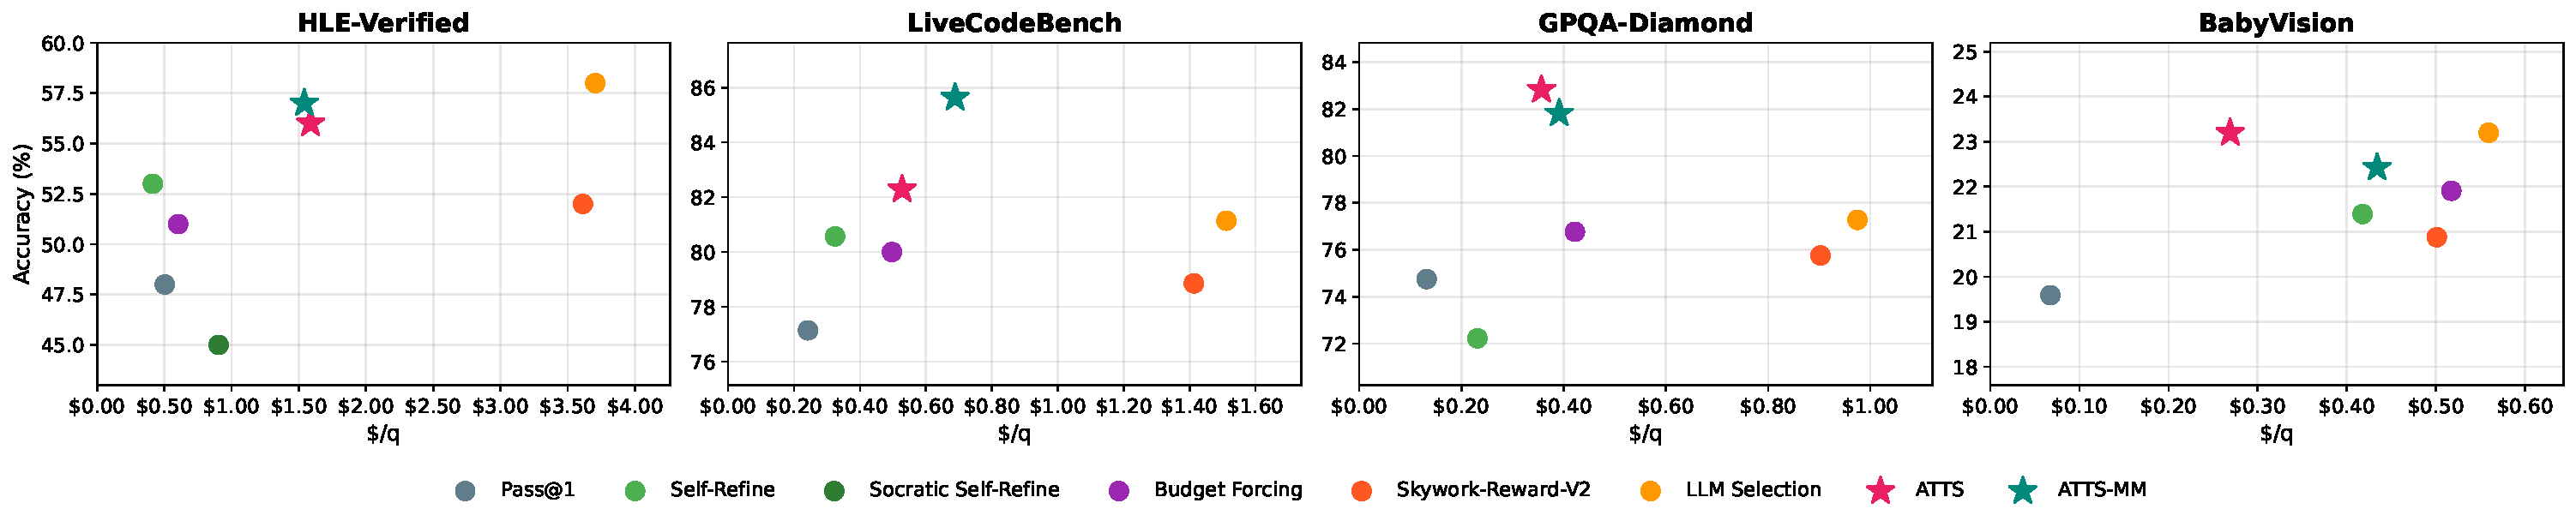
\includegraphics[width=\textwidth]{figures/main_cost_vs_accuracy.pdf}
\caption{Cost-accuracy tradeoffs across the four main benchmarks (left to right: HLE-Verified, LiveCodeBench, GPQA-Diamond, BabyVision). Star markers denote \our{} and \attsmm{}; circles denote baselines. \our{} achieves competitive or superior accuracy at lower cost across all benchmarks.}
\label{fig:cost-accuracy}
\end{figure}

\paragraph{Overall trends.}
% Corrected: HLE cost ratio 2.4x -> 2.3x (LLM Selection $3.71 / ATTS $1.59 = 2.33).
% Range upper bound: 2.4x -> 2.3x. Lower bound 1.7x unchanged (non-HLE benchmark).
Across all four benchmarks, \our{} achieves the best or tied-best accuracy among test-time scaling methods while costing $1.7$--$2.3\times$ \emph{less} than alternatives of comparable accuracy. The gains are largest where one-shot generation leaves the most headroom: on GPQA-Diamond, \our{} improves over Pass@1 by 6.6 percentage points (74.24\% $\to$ 80.81\%) at \$0.34/q; on LiveCodeBench Hard problems, accuracy rises from 60.00\% to 67.50\%. On easy subtasks where the backbone is already near ceiling (100\% Easy on LiveCodeBench), additional exploration yields no benefit---and \our{} does not waste budget there. Where a higher-cost method edges ahead in accuracy---LLM Selection reaches 58.00\% on HLE versus \our{}'s 56.00\%---it does so at $2.3\times$ the cost. This pattern reflects the adaptive allocation at the core of the framework: explore when the current candidate pool is incomplete or inconsistent, and synthesize once the evidence suffices. The results support our main claim: even a purposefully constrained single-tool interface can turn test-time scaling into a semantic compute-allocation problem rather than a fixed sampling schedule.

\subsection{Ablation Studies}

\paragraph{Medium effort is the best cost-efficiency operating point.}
\attsmm{} exposes an \emph{exploration effort} parameter that controls stopping aggressiveness. Figure~\ref{fig:effort-ablation} shows the cost-accuracy tradeoff at three effort levels (Low, Medium, High) across all four benchmarks, holding the model pool and budget fixed; the raw numbers are in Appendix~\ref{app:ablation-data}, Table~\ref{tab:effort-ablation}. The Low-to-Medium transition yields the largest accuracy gain on every benchmark (up to +13 points on HLE, +8.6 on LiveCodeBench). Medium-to-High provides diminishing returns: on LiveCodeBench and BabyVision accuracy is flat while cost nearly doubles; only on HLE-Verified does High effort produce a meaningful further improvement (+3 points). Medium effort therefore represents the best cost-efficiency operating point across the benchmark suite.

\begin{figure}[H]
\centering
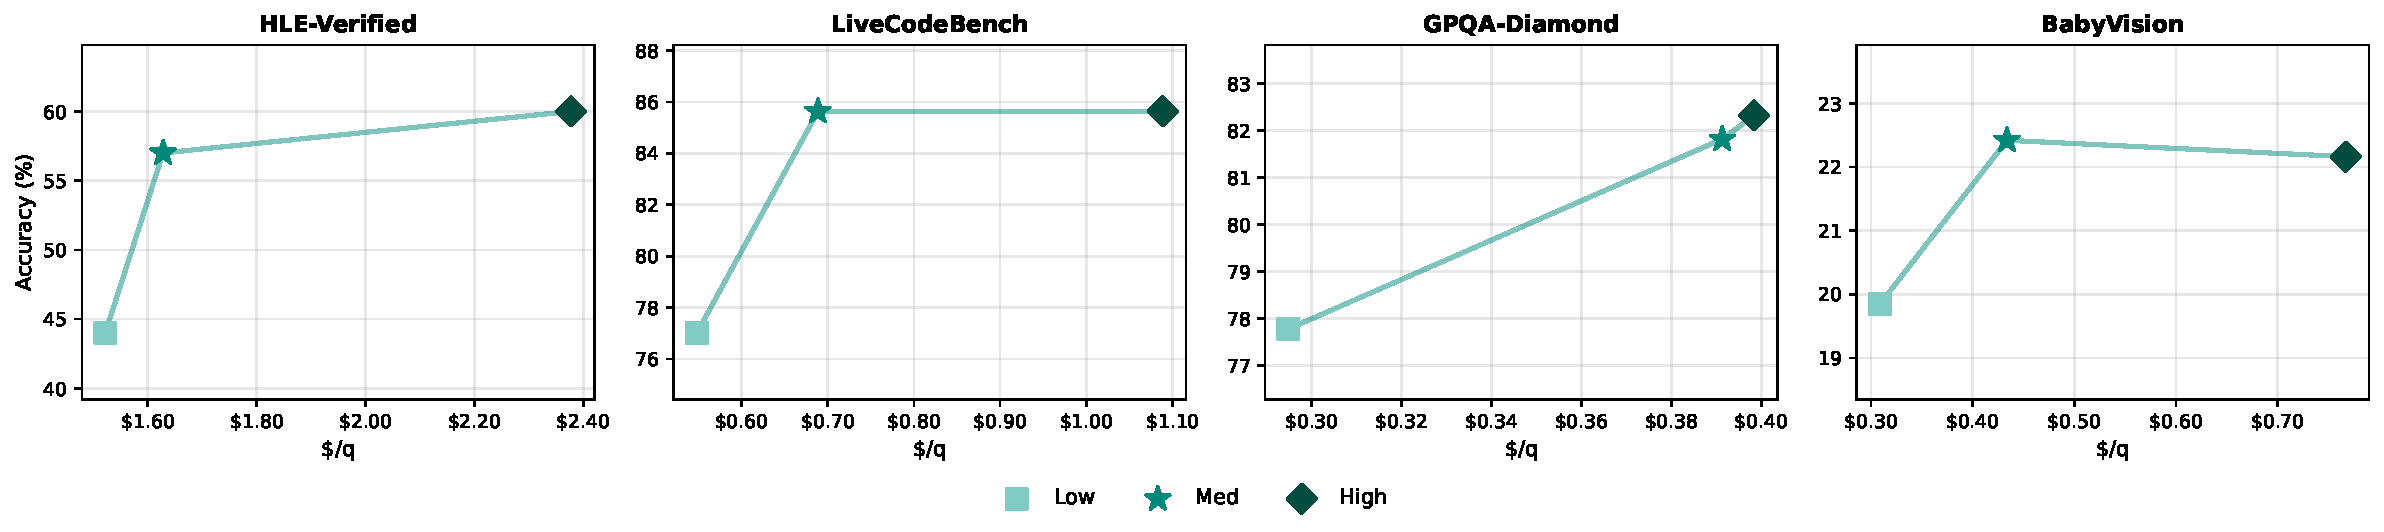
\includegraphics[width=\textwidth]{figures/effort_ablation.pdf}
\caption{Effect of exploration effort on \attsmm{}. Each panel shows the cost-accuracy tradeoff for Low, Medium, and High effort on one benchmark. The steep Low-to-Medium gain and flat Medium-to-High plateau are consistent across all benchmarks.}
\label{fig:effort-ablation}
\end{figure}

\paragraph{Stateful orchestration outperforms separate integration.}
By default, \our{} has the orchestrator produce the final answer directly from its accumulated evidence after deciding to stop exploring. We also evaluate \our{} (+ Integrator), a variant that adds a dedicated \integrate{} step: a separate model call that receives all candidates and synthesizes the final answer independently.

\begin{table}[H]
\centering
\caption{Effect of adding a separate integrator. \our{} has the orchestrator synthesize directly; \our{} (+ Integrator) delegates synthesis to a separate model call.}
\label{tab:integrator-ablation}
\small
\setlength{\tabcolsep}{4pt}
\begin{tabular}{l r r r r}
\toprule
 & \multicolumn{2}{c}{\our{}} & \multicolumn{2}{c}{\our{} (+ Integrator)} \\
\cmidrule(lr){2-3}\cmidrule(lr){4-5}
 & Acc. (\%) & \$/q & Acc. (\%) & \$/q \\
\midrule
% Corrected: Default $1.90->$1.59, +Integrator $2.66->$2.35.
% Both consume 4 bad explores from hle/sonnet/gold cache -> -$31.68 each.
HLE-Verified & 56.00 & 1.59 & 57.00 & 2.35 \\
LiveCodeBench & 82.29 & 0.53 & 80.57 & 0.72 \\
BabyVision & 23.20 & 0.27 & 23.20 & 0.38 \\
GPQA-Diamond & 80.81 & 0.34 & 76.14 & 0.44 \\
\bottomrule
\end{tabular}
\end{table}

Across all four benchmarks, adding a separate integrator does \emph{not} consistently improve accuracy and \emph{always} increases cost (Table~\ref{tab:integrator-ablation}). On GPQA-Diamond, accuracy drops from 80.81\% to 76.14\%; on LiveCodeBench, from 82.29\% to 80.57\%.
% Corrected: $2.66->$2.35, $1.90->$1.59 (compaction-failed explores zeroed).
On HLE-Verified, \our{} (+ Integrator) gains 1 point (57.00\% vs.\ 56.00\%) but at substantially higher cost (\$2.35/q vs.\ \$1.59/q). The degradation likely stems from the integrator having \emph{less} context for synthesis: it only sees the final candidate pool in a single-turn call, whereas the orchestrator has observed the full multi-turn conversation including each candidate's arrival and the reasoning behind its own exploration decisions.

\paragraph{Orchestrator effectiveness is task-dependent, not capability-monotonic.}
We ablate the orchestrator model while keeping the explorer fixed at Sonnet 4.6 (Table~\ref{tab:orch-ablation}, Figure~\ref{fig:orch-ablation}). The results show no monotonic relationship between model strength and orchestrator effectiveness: Opus achieves the highest accuracy on HLE (59\%) and LiveCodeBench (83.4\%), but drops to 77.16\% on GPQA---\emph{below} Sonnet's 80.81\%. Haiku performs comparably to Sonnet on HLE (57\% vs.\ 56\%).

These differences are not explained by stopping behavior. All three orchestrators use similar numbers of explores on each benchmark (e.g.\ 2.15--2.43 on GPQA) and read from the same candidate cache. The gap is therefore attributable to synthesis quality: given similar evidence, the orchestrators produce different final answers. The pattern is \emph{benchmark-dependent} rather than \emph{capability-monotonic}---the strongest model is the best orchestrator on some benchmarks but the \emph{worst} on others. This indicates that orchestrator effectiveness depends on a task-specific interaction between the model's reasoning style and domain characteristics, not simply on model capability. Identifying the precise mechanism underlying this interaction remains an open question.

\begin{figure}[H]
\centering
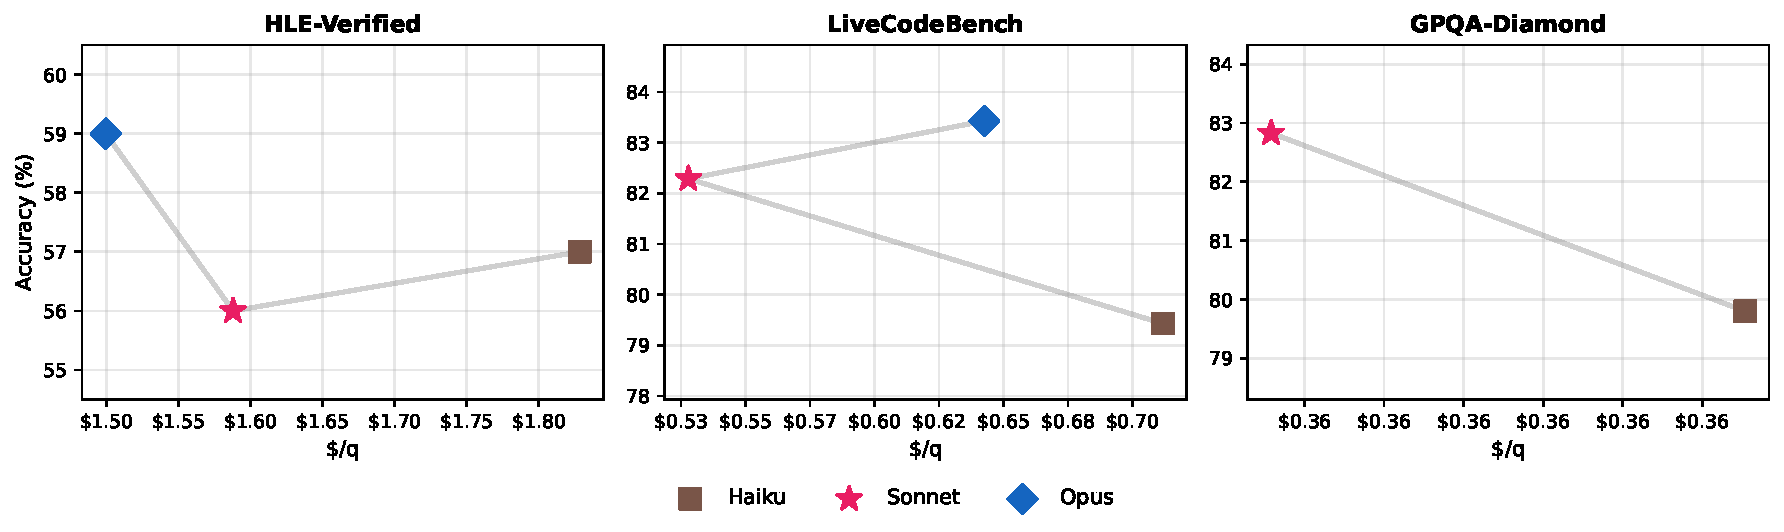
\includegraphics[width=0.9\textwidth]{figures/orch_ablation.pdf}
\caption{Effect of orchestrator model on \our{} accuracy and cost. Haiku is cheapest per call but over-explores, increasing total cost. Opus improves accuracy on HLE and LiveCodeBench but not on GPQA.}
\label{fig:orch-ablation}
\end{figure}

\paragraph{The framework generalizes across model families.}
To evaluate whether \our{} generalizes beyond a single model family, we run the full framework using GPT-5.2 (OpenAI) as the backbone for all three roles---orchestrator, explorer, and synthesizer---keeping the same exploration budget ($T{=}8$) and prompts as the Claude Sonnet configuration. We evaluate on two benchmarks (HLE-Verified and GPQA-Diamond) and test two reasoning effort levels to assess the effect of orchestrator reasoning depth.

\begin{table}[H]
\centering
\caption{Backbone model ablation. All configurations are \our{} with identical prompts and exploration budget. Reasoning effort controls the orchestrator's internal chain-of-thought budget. Gain = Acc. $-$ Pass@1.}
\label{tab:backbone-ablation}
\small
\setlength{\tabcolsep}{3pt}
\begin{tabular}{l l l r r r r}
\toprule
Backbone & Effort & Benchmark & Pass@1 & Acc. & Gain & \$/q \\
\midrule
% Corrected: $1.90->$1.59 (4 compaction-failed explores zeroed, same as Table 1).
Claude Sonnet 4.6 & default & HLE & 48.00 & 56.00 & +8.0 & 1.59 \\
Claude Sonnet 4.6 & default & GPQA & 74.24 & 80.81 & +6.6 & 0.34 \\
\midrule
GPT-5.2 & high & HLE & 55.00 & 57.00 & +2.0 & 0.26 \\
GPT-5.2 & high & GPQA & 56.06 & \textbf{71.07} & \textbf{+15.0} & \textbf{0.16} \\
\midrule
Qwen3.6-35B-A3B-FP8 & default & HLE & 19.00 & 24.00 & +5.0 & 0.013 \\
Qwen3.6-35B-A3B-FP8 & default & GPQA & 72.73 & 84.85 & +12.1 & 0.00 \\
\bottomrule
\end{tabular}
\end{table}

\our{} produces positive gains on both benchmarks for both model families (Table~\ref{tab:backbone-ablation}). On GPQA-Diamond, GPT-5.2 shows the largest absolute gain: +15.0 points over Pass@1 (56.06\% $\to$ 71.07\%), compared to Claude Sonnet's +6.6 points. The lower GPT-5.2 Pass@1 (56.06\% vs.\ the 90.3\% reported for GPT-5.2 in the GPQA leaderboard) reflects the use of \texttt{effort=low} for exploration, which limits reasoning tokens; the orchestrator operates at \texttt{effort=high} during synthesis. % Corrected: $1.59/$0.26 = 6.12 -> 6.1x (was $1.90/$0.26 = 7.31 -> 7.3x).
On HLE-Verified, the gain is smaller (+2.0 points) but still positive, and
the cost is $6.1\times$ lower than Claude. These results demonstrate that \our{}'s adaptive exploration framework is not specific to any model family: the same prompts and control logic transfer to a different provider with consistent gains at substantially lower cost.

\paragraph{Orchestrator reasoning contributes to synthesis quality.}
We ablate the orchestrator's internal reasoning by disabling extended thinking (chain-of-thought) while keeping all other parameters identical: same model (Sonnet 4.6), same cached explores, same exploration budget ($T{=}8$), and same prompts. Without extended thinking, the orchestrator can still read candidate results, call tools, and submit answers---but cannot reason internally between turns.

\begin{table}[H]
\centering
\caption{Effect of disabling orchestrator extended thinking on GPQA-Diamond. All other parameters are held constant. The orchestrator uses the same cached Sonnet explores in both conditions.}
\label{tab:thinking-ablation}
\small
\begin{tabular}{l r r r}
\toprule
Condition & Acc. (\%) & \$/q & Explores/q \\
\midrule
\our{} & 82.83 & 0.35 & 2.15 \\
\our{} (no thinking) & 79.29 & 0.36 & 2.08 \\
\bottomrule
\end{tabular}
\end{table}

\our{} (no thinking) reduces accuracy by 3.5 points relative to \our{} (82.83\% $\to$ 79.29\%) with no cost savings (Table~\ref{tab:thinking-ablation}). The exploration behavior is nearly identical (2.08 vs.\ 2.15 explores per question), indicating that the accuracy gap is attributable to synthesis quality, not stopping behavior. This result confirms that the orchestrator's internal reasoning---even when constrained to a pure orchestration role with no direct problem-solving---contributes meaningfully to evidence evaluation and answer selection.

\section{Limitations}

\our{} has four principal limitations. First, it can only synthesize evidence present in the candidate pool: if all candidates share the same misconception, the orchestrator cannot recover. Second, the framework provides no formal guarantees for stopping optimality, calibration, or budget efficiency; the orchestrator remains a learned heuristic. In practice, the orchestrator converges early: on GPQA, 82\% of questions use exactly two \explore{} calls before stopping, even though the oracle best-of-$N$ curve continues to climb through $N{=}8$. This conservative stopping leaves accuracy on the table, and learning a better stopping criterion remains an open problem. Third, \our{} increases latency and cost relative to direct generation on easy problems where exploration is unnecessary. Finally, the evaluation covers reasoning benchmarks with fixed answer interfaces, not open-ended tool-use agents; the results are evidence about reasoning-oriented test-time scaling, not a complete account of agentic decision-making. We additionally note that on a small fraction of questions ($6$ out of $860$ across the four benchmarks; see Figure~\ref{fig:explore-distribution-all}) the orchestrator produces an answer without issuing any \explore{} call, despite the prompt directing it to invoke \explore{} before synthesizing; the prompt is designed to suppress this behavior and the residual exceptions do not materially affect the aggregate results.

\section{Conclusion}

The central empirical finding of this work is that an LLM orchestrator performing closed-loop decision-making over a minimal action space---a single \explore{} tool---achieves competitive or superior accuracy to fixed-budget test-time scaling strategies while using substantially fewer API calls. \attsmm{} further improves to 57.00\% and 85.63\% on HLE-Verified and LiveCodeBench respectively. The ablation results sharpen this finding: removing the orchestrator's multi-turn context by delegating synthesis to a separate call degrades or fails to improve accuracy on three of four benchmarks, demonstrating that \emph{stateful evidence management}---not just candidate diversity---drives the gains. For the broader field, these results indicate that test-time compute allocation is better approached as closed-loop decision-making by an LLM agent---with an extensible action space over solver dispatch---than as explicit tree search or fixed sampling. A key limitation is the orchestrator's conservative stopping behavior: on GPQA-Diamond, 82\% of questions use exactly two \explore{} calls, leaving substantial headroom relative to oracle best-of-$N$. Learning stopping policies that better exploit the full exploration budget remains an open problem. Code and cached experimental artifacts are available at \url{https://github.com/t2ance/ATTS}.

\bibliographystyle{plainnat}
\bibliography{main}

%%%%%%%%%%%%%%%%%%%%%%%%%%%%%%%%%%%%%%%%%%%%%%%%%%%%%%%%%%%%

\appendix

\section{Implementation Details}
\label{app:implementation-details}

\paragraph{Controller and backend setup.}
\our{} is implemented as a delegated controller with two roles: an orchestrator and an explorer. The orchestrator never solves the task directly; it only decides whether to spend the remaining budget on another \explore{} call or to stop and synthesize the final answer from the accumulated evidence. Each \explore{} call returns a structured candidate containing an answer, supporting reasoning, an approach summary, and an optional confidence score. When the orchestrator decides to stop, it produces the final answer directly via the SDK's structured output mechanism. For the Claude implementation, we use the Claude Agent SDK \citep{claude_agent_sdk} and expose \explore{} as the only available delegated tool. We also evaluate a variant that adds a separate \integrate{} tool that delegates final synthesis to a dedicated model call; see the ablation in Section~4.3. The same high-level controller is reused across benchmarks, while the underlying sub-model backend can be swapped without changing the controller logic.

\paragraph{Prompt families.}
\our{} uses two prompt families: a benchmark-agnostic orchestrator prompt and a benchmark-specific explorer prompt. The orchestrator prompt defines the controller role and explicitly instructs it not to solve the task itself. The explorer prompt asks for an independent solution from scratch under the target answer format. Representative prompt excerpts are shown in Listings~\ref{lst:orchestrator-prompt} and \ref{lst:solver-prompts}. For Claude runs, these prompts are paired with structured-output schemas so that each sub-call returns machine-readable fields rather than free-form text only.

\begin{lstlisting}[
  frame=shadowbox,
  backgroundcolor=\color{gray!5},
  rulecolor=\color{blue!40!black},
  basicstyle=\scriptsize\ttfamily,
  breaklines=true,
  captionpos=b,
  caption={Orchestrator system prompt for \our{} (explore-only). The same principles and examples are shared by \our{} (+ Integrator) and \attsmm{}; only the finalize instruction differs.},
  label={lst:orchestrator-prompt}
]
You are a meta-reasoning orchestrator. You manage a pool of candidate solutions for a problem.

After each explore, you will see the candidate result (answer, confidence, approach, reasoning).

Your final answer must be derived from candidate outputs. You may combine insights from multiple candidates, but you cannot introduce information that no candidate provided.

## Principles (HIGHEST PRIORITY)

1. You cannot solve problems yourself. Your only window into the problem is what solvers return. Reasoning about the problem content constitutes solving.
2. A single candidate, regardless of confidence, does not constitute sufficient evidence. Self-reported confidence is poorly calibrated.
3. Genuine convergence means independent solvers arriving at the same answer through different methods. Shared reasoning paths may reflect shared misconceptions.
4. Solver failure (timeout, empty answer) reflects problem difficulty. Repeated failures mean the problem is practically unsolvable.
5. CRITICAL: Each explore costs budget. Giving up is valid and preferred -- submit empty answer rather than wasting budget.

[6 worked examples follow, showing: starting exploration, disagreement resolution, timeout handling, escalation, and giving up.]
\end{lstlisting}

\begin{lstlisting}[
  frame=shadowbox,
  backgroundcolor=\color{gray!5},
  rulecolor=\color{blue!40!black},
  basicstyle=\scriptsize\ttfamily,
  breaklines=true,
  captionpos=b,
  caption={Orchestrator prompt additions for \attsmm{}. The orchestrator receives model profiles with pricing and benchmark scores, and adapted principles for heterogeneous model selection.},
  label={lst:multi-model-prompt}
]
You have access to multiple solver models of different capability and cost. Each explore call lets you choose which model to use.

## Model Profiles
Pricing (per million tokens): Haiku $1/$5, Sonnet $3/$15, Opus $5/$25.
[Public benchmark scores table: MATH-500, AIME, GPQA, HLE, ARC-AGI-2, SWE-bench, etc.]

## Adapted Principles
3. Candidates from different models that agree provide stronger evidence than same-model candidates.
4. A weaker model failing does not mean a stronger model will also fail. Start cheap, escalate on failure.

## Exploration Effort Constraints (appended to user message)
LOW:    Stop as soon as 2 candidates from any model converge.
MEDIUM: MUST call explore >= 3 times, MUST use >= 2 models.
HIGH:   MUST call explore >= 5 times, MUST use all 3 models.
\end{lstlisting}

\begin{lstlisting}[
  frame=shadowbox,
  backgroundcolor=\color{gray!5},
  rulecolor=\color{blue!40!black},
  basicstyle=\scriptsize\ttfamily,
  breaklines=true,
  captionpos=b,
  caption={Explorer prompt (left) and integrator prompt (right). Both share the same answer format rules enforced via structured output schema field descriptions.},
  label={lst:solver-prompts}
]
Explorer:
You are an expert problem solver. Solve the given problem step by step.
If you cannot solve it exactly, give your best estimate and set confidence accordingly.
Schema: {approach, reasoning, answer, confidence}

Integrator:
You are an expert answer synthesizer. You will receive a problem and multiple candidate solutions.
Your job: (1) Analyze each candidate's reasoning individually, (2) Identify agreements and disagreements, (3) Judge which side has more rigorous reasoning, (4) Point out logical errors, (5) Produce a verified final answer.
Schema: {analysis, final_answer, reasoning}
\end{lstlisting}

\paragraph{Schemas and benchmark-specific prompt instantiation.}
Benchmark-specific adaptation is intentionally lightweight. Most answer-based tasks share the explorer schema \texttt{\{approach, reasoning, answer, confidence\}} and the integrator schema \texttt{\{analysis, final\_answer, reasoning\}}. Only the answer interface changes across tasks. LiveCodeBench uses code-generation fields, GPQA expects one option letter, and multimodal benchmarks pass the associated image with the text question. This design keeps the controller fixed while preserving each benchmark's native answer format and grading protocol.

\paragraph{Runtime behavior.}
At runtime, the controller maintains the candidate pool and repeatedly calls \explore{} until the exploration budget is exhausted or the controller decides to stop and synthesize. The same implementation supports both text-only and image-conditioned tasks, and all runs can optionally record the controller trace and sub-model outputs for later inspection. These choices make the evaluation pipeline inspectable without changing the core decision process.

\paragraph{Grading.}
LiveCodeBench uses deterministic grading via code execution. GPQA-Diamond uses exact option-letter matching, consistent with the official GPQA evaluation protocol~\citep{gpqa_paper}; as with any regex-based extraction, minor formatting variations in model output may introduce small amounts of grading noise. HLE-Verified and BabyVision use an LLM judge (Claude Haiku 4.5) that compares the predicted answer against the reference answer.

\paragraph{Baseline implementations.}
All baselines use the same backbone model and the same benchmark-specific answer format as \our{}, so the comparison isolates the inference-time strategy.

\emph{Pass@1} generates a single independent response per question and returns its answer directly.

\emph{Majority Voting} draws \(N=8\) independent responses and selects the most frequent answer.

\emph{Self-Refine}~\citep{self_refine_paper} generates an initial draft, then enters a feedback-revision loop: a separate feedback call critiques the current draft and returns a correctness judgment; if the draft is judged incorrect, a revision call produces an updated draft conditioned on all prior drafts and feedbacks. The loop terminates when feedback returns a positive judgment or the iteration budget is exhausted. In practice, the feedback model frequently accepts the initial draft, so Self-Refine terminates after a single feedback call on the majority of questions, which explains its relatively low cost on most benchmarks.

\emph{Socratic Self-Refine}~\citep{socratic_self_refine_paper} replaces the Self-Refine feedback step with a Socratic-style probing pass: instead of producing a free-form critique, the feedback call generates a structured list of probing questions that target the current draft's reasoning, and the revision call must answer those questions while updating the draft. The same iteration budget and termination condition as Self-Refine are used. The probing-question step adds an extra model call per iteration relative to Self-Refine, so per-question cost is somewhat higher even though stopping behavior is similar. The intuition is that explicitly grounding the revision in answered probes should reduce the rate at which the model rubber-stamps the initial draft; in our results this shows up as a small accuracy improvement on LiveCodeBench (where reasoning depth helps most) and as a small accuracy regression on HLE-Verified (where the additional probes occasionally talk the model out of an originally correct answer).

\emph{Budget Forcing}~\citep{s1_budget_forcing_paper} runs \(N\) sequential rounds on the same question. Round~1 generates an initial solution. Each subsequent round feeds the previous round's full reasoning trace back to the model with ``Wait'' appended, suppressing premature termination and forcing the model to continue deliberating before producing a new answer. All \(N\) rounds run unconditionally, and the final round's answer is returned. Because continuation rounds extend the existing reasoning rather than solving from scratch, they tend to produce shorter completions and lower per-round cost.

\emph{Reward-model reranking} (Skywork-Reward-V2 for text benchmarks, VisualPRM for multimodal benchmarks) draws the same \(N=8\) independent candidates, then scores each with a separately trained reward model and returns the highest-scoring answer. Skywork-Reward-V2 is an outcome reward model that assigns a single scalar score per response; VisualPRM is a process reward model that aggregates per-step scores. The reward models run locally and incur no API cost, but the candidate generation cost is identical to that of Majority Voting.

\section{Ablation Data}
\label{app:ablation-data}

\begin{table}[H]
\centering
\caption{Effect of exploration effort on \attsmm{}. Accuracy (\%) and average cost per question (\$/q) across benchmarks.}
\label{tab:effort-ablation}
\small
\setlength{\tabcolsep}{4pt}
\begin{tabular}{l r r r r r r}
\toprule
 & \multicolumn{2}{c}{\attsmm{} (Low)} & \multicolumn{2}{c}{\attsmm{}} & \multicolumn{2}{c}{\attsmm{} (High)} \\
\cmidrule(lr){2-3}\cmidrule(lr){4-5}\cmidrule(lr){6-7}
 & Acc. & \$/q & Acc. & \$/q & Acc. & \$/q \\
\midrule
% Corrected: Low $1.52->$1.44, Med $1.63->$1.54. Each consumed 1 bad explore (-$8.63).
% High $2.38 unchanged (0 bad explores consumed).
HLE-Verified & 44.00 & 1.44 & 57.00 & 1.54 & 60.00 & 2.38 \\
LiveCodeBench & 77.01 & 0.55 & 85.63 & 0.69 & 85.63 & 1.09 \\
BabyVision & 19.85 & 0.31 & 22.42 & 0.43 & 22.16 & 0.77 \\
GPQA-Diamond & 77.78 & 0.29 & 81.82 & 0.39 & 82.32 & 0.40 \\
\bottomrule
\end{tabular}
\end{table}

\begin{table}[H]
\centering
\caption{Effect of orchestrator model on \our{} accuracy (\%) and cost (\$/q). Explorer is Sonnet 4.6 throughout.}
\label{tab:orch-ablation}
\small
\setlength{\tabcolsep}{4pt}
\begin{tabular}{l r r r r r r}
\toprule
 & \multicolumn{2}{c}{\our{} (Haiku orch)} & \multicolumn{2}{c}{\our{}} & \multicolumn{2}{c}{\our{} (Opus orch)} \\
\cmidrule(lr){2-3}\cmidrule(lr){4-5}\cmidrule(lr){6-7}
 & Acc. & \$/q & Acc. & \$/q & Acc. & \$/q \\
\midrule
% Corrected: Haiku $2.23->$1.83 (5 bad consumed, -$40.28).
% Sonnet $1.90->$1.59 (4 bad consumed, -$31.68). Opus $1.79->$1.50 (3 bad consumed, -$28.75).
% All three orchestrators read from hle/sonnet/gold cache; different consumption due to stopping.
HLE-Verified & 57.00 & 1.83 & 56.00 & 1.59 & 59.00 & 1.50 \\
LiveCodeBench & 79.43 & 0.71 & 82.29 & 0.53 & 83.43 & 0.64 \\
GPQA-Diamond & 80.20 & 0.36 & 80.81 & 0.34 & 77.16 & 0.34 \\
\bottomrule
\end{tabular}
\end{table}

\section{Qualitative Analysis}
\label{app:case-studies}

To understand \emph{how} \our{} improves over Pass@1, we examine the 22 GPQA-Diamond questions where \our{} produces a correct answer but the first exploration does not. Table~\ref{tab:success-types} categorizes these by the orchestrator's mechanism of improvement.

\begin{table}[H]
\centering
\caption{How \our{} improves over Pass@1 on GPQA-Diamond. \emph{Majority correction}: multiple explores converge on the correct answer, overriding an incorrect first candidate. \emph{Minority extraction}: the orchestrator identifies a correct minority candidate by evaluating reasoning quality. In one question, \our{} changes a correct Pass@1 answer to an incorrect one.}
\label{tab:success-types}
\small
\begin{tabular}{l r r}
\toprule
Orchestrator behavior & Count & Fraction \\
\midrule
Majority correction & 18 & 82\% \\
Minority extraction & 4 & 18\% \\
\midrule
Total rescued (Pass@1 wrong $\to$ \our{} correct) & 22 & \\
Total hurt (Pass@1 correct $\to$ \our{} wrong) & 1 & \\
\textbf{Net gain} & \textbf{+21} & \\
\bottomrule
\end{tabular}
\end{table}

Most improvements (82\%) arise from the diversity of independent explorations: when the first candidate is wrong, subsequent explorations are likely to find the correct answer, and the orchestrator follows the emerging consensus. The remaining 18\% involve the orchestrator overriding the explore majority based on reasoning quality---a capability that goes beyond simple voting. Listings~\ref{lst:majority-case} and~\ref{lst:minority-case} show representative examples of each mechanism.

\begin{lstlisting}[
  frame=shadowbox,
  backgroundcolor=\color{gray!5},
  rulecolor=\color{blue!40!black},
  basicstyle=\scriptsize\ttfamily,
  breaklines=true,
  captionpos=b,
  caption={Majority correction: a Diels-Alder/NMR problem (GPQA-Diamond). The first explore gives the wrong answer (D); subsequent explores converge on A through independent analyses. The orchestrator follows the consensus.},
  label={lst:majority-case}
]
Question: A dicarboxylic acid containing a cis-alkene was dehydrated to
the corresponding anhydride [...] reacted with 1,2,3,4-tetramethyl-
cyclopentadiene [...] How many peaks are in the CHCH3 region?
Options: (A) 2 peaks  (B) 3 peaks  (C) 4 peaks  (D) 8 peaks
Gold: A

Explore #1: answer=D, confidence=0.85
  Approach: Identify anhydride, determine Diels-Alder stereochemistry.

Explore #2: answer=A, confidence=0.88
  Approach: Maleic anhydride + tetramethylcyclopentadiene gives endo
  bicyclo[2.2.1] product. The methyl groups split into two sets by
  symmetry: bridge methyls (6H singlet) and ring methyls (6H singlet).

Explore #3: answer=A, confidence=0.88
  [Independent confirmation via the same endo-selectivity argument.]

Orchestrator synthesis (after 5 explores, 3 favoring A):
  "Three independent explorations converged on A through consistent
   analysis of the endo product's symmetry. The dissenting candidates
   incorrectly assumed exo selectivity."
  Final answer: A, confidence=0.75. CORRECT.
\end{lstlisting}

\begin{lstlisting}[
  frame=shadowbox,
  backgroundcolor=\color{gray!5},
  rulecolor=\color{blue!40!black},
  basicstyle=\scriptsize\ttfamily,
  breaklines=true,
  captionpos=b,
  caption={Minority extraction: a molecular symmetry problem (GPQA-Diamond). The explore majority (4/7) favors molecule A, but the orchestrator identifies a flaw in the majority's reasoning and selects the minority answer B.},
  label={lst:minority-case}
]
Question: Which of the following molecules has C3h symmetry?
(A) Triisopropyl borate  (B) Triphenylene trianhydride
(C) Benzene trianhydride  (D) Quinuclidine
Gold: B

Explore #1: answer=A, confidence=0.92
  "Triisopropyl borate: B is sp2 planar, C3 axis + sigma_h from the
   BO3 plane, no C2 or sigma_v. Point group: C3h."
Explore #2: answer=B, confidence=0.85
  "Triisopropyl borate: isopropyl groups adopt a propeller arrangement
   -- not planar, so no sigma_h. True point group: C3, not C3h."
Explore #3: answer=A, confidence=0.88
  [Repeats the sp2-planar argument for molecule A.]
Explore #4: answer=B, confidence=0.82
  [Identifies that benzene trianhydride (C) has 3 perpendicular C2
   axes -> D3h, while triphenylene trianhydride (B) lacks C2 due to
   inequivalent positions in the fused ring system -> C3h.]
[... 3 more explores: 2 favor A, 1 favors B. Final tally: A=4, B=3.]

Orchestrator synthesis (after 7 explores):
  "The candidates favoring A assume the isopropyl groups preserve
   sigma_h, but Explore #4 correctly notes that the propeller
   conformation breaks this plane. Triphenylene trianhydride (B) has
   C3h intrinsic to its rigid topology -- positions 1,2 in triphenylene
   are inequivalent, preventing C2 axes that would elevate to D3h."
  Final answer: B, confidence=0.62. CORRECT.
\end{lstlisting}

\paragraph{Emergent behavior: selective exploration bypass.}
When using Opus 4.6 as orchestrator, we observe a distinct behavior absent in weaker models: the orchestrator occasionally bypasses exploration entirely, answering directly from its own knowledge. On GPQA-Diamond, Opus skips exploration on 30 of 198 questions (15\%), achieving 90\% accuracy on these self-answered questions---substantially higher than its 75\% accuracy on explored questions. This suggests that stronger orchestrators develop an implicit sense of which problems are within their direct competence, selectively invoking the exploration mechanism only when needed.

\section{Benchmark Details}
\label{app:benchmark-details}

\paragraph{HLE-Verified.}\label{app:hle-details}
We use the official HLE-Verified dataset release \texttt{skylenage/HLE-Verified} \citep{hle_verified_dataset_hf}, which partitions the 2,500 audited HLE items into Gold (668), Revision (1,143), and Uncertain (689) subsets \citep{hle_verified_paper}. HLE-Verified preserves the original HLE answer-based evaluation semantics: each item contains a problem statement, a final answer, and sometimes a rationale, but official scoring is driven by the problem and final answer, with rationale used only as auxiliary evidence during verification and revision \citep{hle_paper_nature,hle_verified_paper}. In the HLE-Verified evaluation paper, the reported baselines are run on the text-only portion of HLE using the official HLE system prompt, each model's default recommended decoding configuration, and five independent rollouts per item; the paper reports both \emph{avg5 Accuracy} and \emph{Calibration Error}, with calibration computed by the official HLE evaluation code \citep{hle_verified_paper}. In this paper, HLE reporting is aligned to the Gold-subset setting, while Table~\ref{tab:main-results}(a) reproduces the official revised-subset accuracy references from \citet{hle_verified_paper} for context. Our grading uses an LLM-as-judge pipeline with Claude Haiku 4.5 as the judge model, which determines semantic equivalence between the predicted and gold answers.

\paragraph{LiveCodeBench.}\label{app:lcb-details}
We use the LiveCodeBench code generation release \texttt{livecodebench/code\_generation\_lite} \citep{lcb_dataset_hf}, configuration \texttt{v6} \citep{livecodebench_paper}. LiveCodeBench is a continuously updated programming benchmark sourced from LeetCode, AtCoder, and CodeForces. Each problem is tagged by release date, so official evaluations can be restricted to post-cutoff time windows for contamination-aware comparison \citep{livecodebench_paper}. In the official code generation setting, the model receives the natural-language problem statement together with example input-output pairs and must return a complete executable program. Correctness is determined purely by functional correctness on unseen tests, using the benchmark harness rather than an LLM judge \citep{livecodebench_paper}. The benchmark paper reports \emph{Pass@1} as the primary metric and also reports difficulty-stratified \emph{Pass@1} using the platform-provided Easy/Medium/Hard labels. The public generation leaderboard \citep{livecodebench_leaderboard} follows this same framing, and Table~\ref{tab:main-results}(b) therefore reports overall and difficulty-wise Pass@1 from the same leaderboard view. Our grading uses the official \texttt{lcb\_runner} execution harness with a 10-second per-test-case timeout.

\paragraph{BabyVision.}\label{app:babyvision-details}
We use the BabyVision dataset release \texttt{UnipatAI/BabyVision} \citep{babyvision_dataset_hf}, which contains 388 image-question pairs spanning four task families: Fine-grained Discrimination (163), Visual Tracking (83), Spatial Perception (91), and Visual Pattern Recognition (51) \citep{babyvision_paper}. The benchmark contains 135 multiple-choice items and 253 fill-in-the-blank items; in the official inference setup, each model is queried with a unified prompt template of the form ``\texttt{\{question\} Think about the question and give your final answer in \{format\}.}'', which standardizes answer formatting for downstream extraction and judging \citep{babyvision_paper}. Official scoring uses an LLM-as-judge pipeline: given a model answer and the gold answer, Qwen3-Max determines semantic equivalence under the benchmark's fixed judge prompt, which the authors report as having perfect agreement with their human evaluators on the benchmark responses they audited \citep{babyvision_paper}. The primary metric is \emph{Avg@3}, defined in the paper as the mean \emph{Pass@1} accuracy across three random runs, and the official tables additionally report the corresponding standard deviation; Table~\ref{tab:main-results}(c) follows the official overall-plus-family breakdown but keeps only the mean scores in the main text table. Our grading uses an LLM-as-judge pipeline with Claude Haiku 4.5 as the judge model, following the same semantic equivalence protocol as the official evaluation but substituting the judge model.

\paragraph{GPQA-Diamond.}\label{app:gpqa-details}
We use the GPQA release \texttt{Idavidrein/gpqa} \citep{gpqa_dataset_hf}, configuration \texttt{gpqa\_diamond}, which corresponds to the 198-question Diamond subset introduced in the GPQA paper \citep{gpqa_paper}. GPQA is a graduate-level four-option multiple-choice science benchmark spanning biology, physics, and chemistry, and GPQA-Diamond is the highest-stringency subset retained after expert-accuracy and non-expert-difficulty filtering \citep{gpqa_paper}. The official task is closed-book answer selection unless otherwise stated: the model is shown the question and four candidate options and must output exactly one final option. Scoring is exact option-key accuracy with no semantic judge and a random-guess baseline of \(25\%\) \citep{gpqa_paper}. In addition to Diamond-set accuracy, the original GPQA paper also reports accuracies on the Extended and Main sets and distinguishes closed-book few-shot/CoT baselines from an open-book GPT-4-with-search baseline; Table~\ref{tab:main-results}(d) keeps the main-text comparison focused on the Diamond-set accuracy column used by current public references. Our grading extracts the option letter (A--D) from the model response via regex and performs exact matching against the gold option key, with no LLM judge, consistent with the official protocol.

\section{Supplementary Benchmark: RBench-V}
\label{app:rbenchv}

This appendix adds a supplementary evaluation on RBench-V \citep{rbenchv_paper}, a visual reasoning benchmark with multi-modal outputs. RBench-V is not part of the four main-text benchmarks because the official RBench-V protocol scores not only the final textual answer but also intermediate image generations (e.g., auxiliary lines drawn into the input figure). Most current API models---including the orchestrators and explorers used elsewhere in this paper---do not natively emit raster images during reasoning, so direct comparison against published RBench-V leaderboard rows requires careful disclosure of this protocol mismatch. We include the benchmark here as a stress test of \our{} on a tasks where the visual reasoning channel itself is the binding capability, rather than as a head-to-head ranking against \citet{rbenchv_paper}.

\paragraph{Dataset and protocol.}\label{app:rbenchv-details}
We use the RBench-V dataset release at \citet{rbenchv_dataset_hf}. The benchmark consists of 803 multi-modal reasoning problems spanning four task families: Math, Physics, Counting, and Games \citep{rbenchv_paper}. Every item is image-conditioned, and the question pool mixes multiple-choice items with open-ended free-form answers. The official RBench-V protocol differentiates two scoring views: \emph{Overall}, which averages over all four families, and \emph{w/o Math}, which excludes the Math subset on the rationale that geometry items in Math admit algebraic shortcuts that bypass the visual reasoning channel and therefore inflate apparent multi-modal capability \citep{rbenchv_paper}. Table~\ref{tab:lb-rbenchv} reports both views together with the four per-family columns, mirroring \citet{rbenchv_paper}'s primary results table. Because the benchmark includes both multiple-choice and open-ended questions, the official protocol grades all items through a unified LLM-as-judge framework with GPT-4o as the judge model, reporting Top-1 accuracy as the primary metric \citep{rbenchv_paper}. Our grading reuses an LLM-as-judge pipeline with Claude Haiku 4.5 in the judge role, preserving the open-ended semantic-equivalence semantics required by the official protocol while substituting the judge backbone for cost and reproducibility reasons. As with the rest of the paper, our explorers receive only the original problem (image plus text) without ground-truth answers; the orchestrator does not attempt to emit images and must reason about the visual content through textual descriptions delegated to its explorers.

\begin{table}[t!]
\centering
\caption{RBench-V leaderboard reference (top group, cited from Table~1 of \citet{rbenchv_paper}) together with aligned reporting rows for the baselines and \our{} (bottom group, our evaluation). All numbers are accuracies (\%); \$/q reflects API token charges only, on the same convention used in Table~\ref{tab:main-results}. ``w/o Math'' excludes the Math subset, which the benchmark authors recommend as a tighter probe of multi-modal reasoning capability \citep{rbenchv_paper}. Bottom-group rows marked \textit{TBD} are pending evaluation; see the deferred-evaluation note at the end of this appendix.}
\label{tab:lb-rbenchv}
\scriptsize
\setlength{\tabcolsep}{3pt}
\begin{tabular}{l r r r r r r r}
\toprule
 & Overall & w/o Math & Math & Physics & Counting & Games & \$/q \\
 & ($n{=}803$) & ($n{=}627$) & ($n{=}176$) & ($n{=}157$) & ($n{=}195$) & ($n{=}275$) & \\
\midrule
Human Experts & 82.3 & 81.7 & 84.7 & 69.4 & 81.0 & 89.1 & -- \\
\midrule
\groupheader{8}{Zero-Shot Models (cited from \citet{rbenchv_paper}, Table~1)}
OpenAI o3 & \textbf{25.8} & \textbf{19.5} & \textbf{48.3} & \textbf{20.4} & \textbf{22.1} & \textbf{17.1} & -- \\
OpenAI o4-mini & 20.9 & 14.6 & 43.2 & 12.7 & 17.4 & 13.8 & -- \\
Gemini 2.5 Pro & 20.2 & 13.9 & 42.6 & 9.6 & 19.0 & 12.7 & -- \\
Doubao-1.5-thinking-pro-m & 17.1 & 11.0 & 38.6 & 13.4 & 9.7 & 10.5 & -- \\
OpenAI o1 & 16.2 & 11.0 & 34.7 & 5.7 & 12.3 & 13.1 & -- \\
Doubao-1.5-vision-pro & 15.6 & 11.5 & 30.1 & 8.9 & 12.8 & 12.0 & -- \\
GPT-4o (2025-03-27) & 14.1 & 11.2 & 24.4 & 3.2 & 13.3 & 14.2 & -- \\
GPT-4.1 & 13.6 & 11.7 & 20.5 & 5.7 & 11.3 & 15.3 & -- \\
\midrule
\groupheader{8}{Test-Time Scaling Methods (our evaluation)}
Pass@1 & \textit{TBD} & \textit{TBD} & \textit{TBD} & \textit{TBD} & \textit{TBD} & \textit{TBD} & \textit{TBD} \\
Majority Voting & \textit{TBD} & \textit{TBD} & \textit{TBD} & \textit{TBD} & \textit{TBD} & \textit{TBD} & \textit{TBD} \\
Self-Refine & \textit{TBD} & \textit{TBD} & \textit{TBD} & \textit{TBD} & \textit{TBD} & \textit{TBD} & \textit{TBD} \\
Budget Forcing & \textit{TBD} & \textit{TBD} & \textit{TBD} & \textit{TBD} & \textit{TBD} & \textit{TBD} & \textit{TBD} \\
VisualPRM & \textit{TBD} & \textit{TBD} & \textit{TBD} & \textit{TBD} & \textit{TBD} & \textit{TBD} & \textit{TBD} \\
LLM Selection ($N{=}8$) & \textit{TBD} & \textit{TBD} & \textit{TBD} & \textit{TBD} & \textit{TBD} & \textit{TBD} & \textit{TBD} \\
\our{} & \textit{TBD} & \textit{TBD} & \textit{TBD} & \textit{TBD} & \textit{TBD} & \textit{TBD} & \textit{TBD} \\
\attsmm{} & \textit{TBD} & \textit{TBD} & \textit{TBD} & \textit{TBD} & \textit{TBD} & \textit{TBD} & \textit{TBD} \\
\bottomrule
\end{tabular}
\end{table}

\paragraph{Deferred-evaluation note.}
The bottom group of Table~\ref{tab:lb-rbenchv} is currently a structural placeholder. Pre-cached explores from the cheaper Claude tier exist for a partial subset of RBench-V items, but a full evaluation matrix matching the eight rows of Table~\ref{tab:main-results}(d) (Pass@1, Majority Voting, Self-Refine, Budget Forcing, VisualPRM, LLM Selection, \our{}, \attsmm{}) has not yet been run. We disclose this gap explicitly here rather than omit the benchmark, so that the structural slot in the appendix exists and the leaderboard reference rows are stable before our own numbers are produced. The reason RBench-V was deferred to the appendix during the main-text revision is the protocol mismatch noted at the start of this section: image-emitting reasoning is part of RBench-V's official capability target but not part of \our{}'s current explorer interface, so a like-for-like ranking against published rows requires care that is out of scope for the main-text comparison.

\section{Explore-Count Distributions}
\label{app:explore-distributions}

Figure~\ref{fig:explore-distribution-all} reports how many model calls each per-question trajectory uses, on each of the four main benchmarks, for \our{} (top row), the Self-Refine baseline (middle row), and the Socratic Self-Refine baseline (bottom row). Each panel is a histogram whose $x$-axis is the number of calls used for a question and whose $y$-axis is the number of questions at that count; bar heights are annotated with the exact counts. Panel titles report the method, the benchmark name, the number of evaluated questions $n$, and the mean number of calls per question.

\begin{figure}[H]
\centering
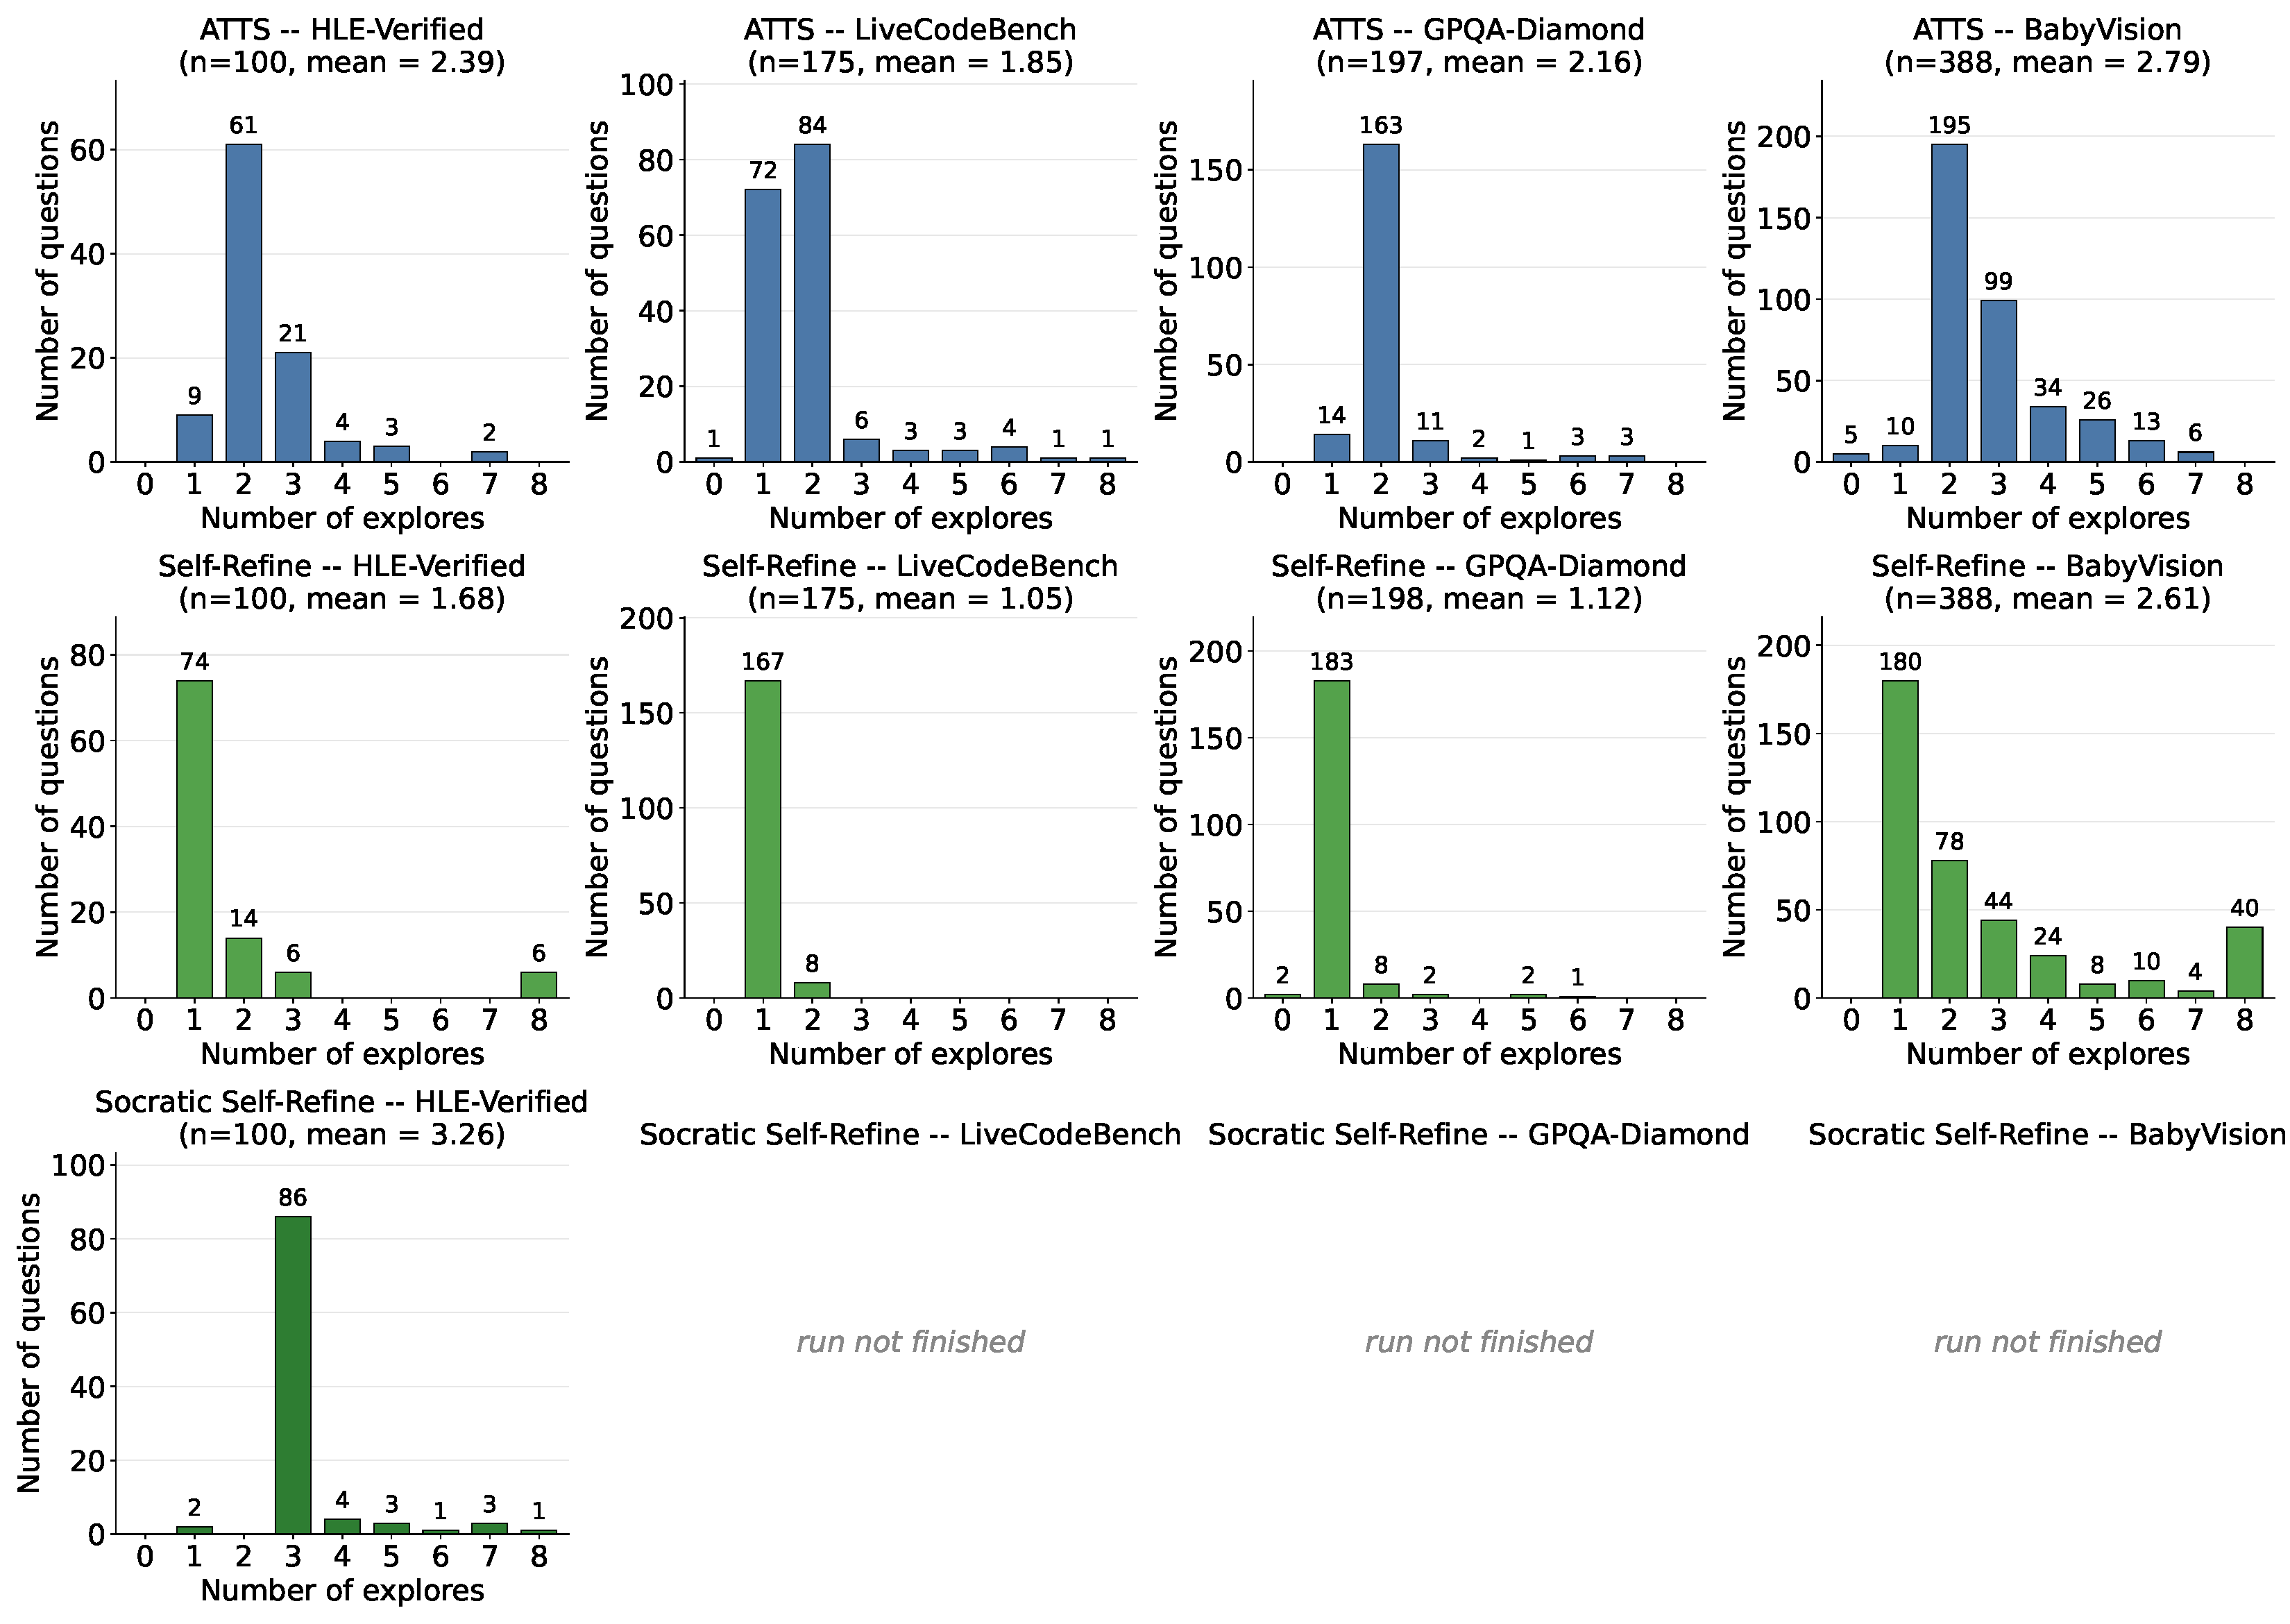
\includegraphics[width=\textwidth]{figures/explore_distribution_all.pdf}
\caption{Per-benchmark distribution of the number of model calls used per question, comparing \our{} (top row, blue), the Self-Refine baseline (middle row, light green), and the Socratic Self-Refine baseline (bottom row, dark green). Columns from left to right: HLE-Verified (Gold subset), LiveCodeBench, GPQA-Diamond, BabyVision. All three rows share the same axes and budget cap $T{=}8$, so differences in the observed distributions reflect each method's stopping mechanism. Bar heights are annotated with exact counts; panel titles include the sample size $n$ and the per-question mean. Budget Forcing is omitted because it terminates only at the cap by construction, so its distribution is degenerate at $T{=}8$.}
\label{fig:explore-distribution-all}
\end{figure}

All four benchmarks share the same exploration budget $T{=}8$ and the same orchestrator prompt, so differences in the observed distributions reflect the orchestrator's input-conditioned stopping decisions rather than externally imposed budgets. We highlight five observations from the top row of this figure, then return to the contrast with Self-Refine.

\paragraph{Observation 1: Mean explore count tracks benchmark difficulty.}
The per-benchmark mean \explore{} count ranges from $1.85$ on LiveCodeBench to $2.79$ on BabyVision, with GPQA-Diamond at $2.16$ and HLE-Verified at $2.39$. Harder benchmarks---those on which test-time scaling methods reach lower absolute accuracy in Table~\ref{tab:main-results}---receive more exploration per question on average. Given that all four benchmarks share the same budget and the same orchestrator prompt, this is a direct numerical expression of the adaptive compute allocation claim: the controller spends more calls where first-pass evidence is less conclusive.

\paragraph{Observation 2: The modal behavior is ``explore twice,'' not ``explore once.''}
Three of the four benchmarks (HLE-Verified, GPQA-Diamond, BabyVision) place their distribution mode at $n{=}2$ \explore{} calls, and the share of questions stopping at $n{=}1$ is below $15\%$ on each of these three benchmarks. LiveCodeBench is the only exception, with a bimodal distribution in which the first mode at $n{=}1$ ($72/175$ questions) is comparable in size to the second mode at $n{=}2$ ($84/175$). The default orchestrator behavior is therefore ``explore twice before synthesizing,'' not ``explore once and submit.'' This empirically counters the assumption that a confidence-based orchestrator collapses exploration to a single call on most questions. The contrast with Self-Refine is sharp: under Self-Refine (Figure~\ref{fig:explore-distribution-all}, bottom row) the mode is $n{=}1$ on three of four benchmarks (mean $1.05$--$1.68$ on HLE/LCB/GPQA) because the critic accepts the initial draft on the first revision check for the vast majority of questions. \our{}'s mass is centered between Self-Refine's one-shot acceptance and a hypothetical fixed-budget schedule, reflecting that the orchestrator's stop decisions are conditioned on accumulated evidence rather than on a single one-shot critic check.

\paragraph{Observation 3: The budget cap $T{=}8$ is almost never reached.}
Across the $860$ questions in the four benchmarks combined, exactly one question consumes the full exploration budget of $T{=}8$ (on LiveCodeBench). Questions using $n \ge 6$ \explore{} calls remain rare on every benchmark: $6$ on LiveCodeBench, $6$ on GPQA-Diamond, $2$ on HLE-Verified, and $19$ on BabyVision. The orchestrator terminates exploration well before the cap on virtually every question, supporting the interpretation that $T$ functions as a safety ceiling rather than a target.

\paragraph{Observation 4: LiveCodeBench bimodality reflects per-problem difficulty recognition.}
LiveCodeBench is the only benchmark with a substantial mass at $n{=}1$ ($41\%$ of questions). These single-explore questions likely correspond to problems for which the first candidate is obviously sufficient: LiveCodeBench's Easy tier already reaches $100\%$ Pass@1 in the main results (Table~\ref{tab:main-results}(b)), and a fraction of Medium problems are similarly unambiguous once a first candidate is produced. The orchestrator's ability to terminate immediately on such problems, rather than always continuing to the modal $n{=}2$ seen on the other three benchmarks, is direct evidence that the controller performs per-problem difficulty recognition rather than following a fixed exploration schedule.

\paragraph{Observation 5: BabyVision is the inverse-pattern case.}
BabyVision is the only benchmark on which the highest mean \explore{} count ($2.79$) co-occurs with the lowest accuracy among the four ($23.20\%$ in Table~\ref{tab:main-results}(c)). The orchestrator explores most aggressively on BabyVision---roughly half of all questions receive three or more \explore{} calls---yet the additional exploration does not translate into accuracy gains, and all test-time scaling methods on this benchmark cluster within a narrow $19$--$23\%$ band. The orchestrator detects that the first candidate is often insufficient and requests more evidence, but the backbone's visual reasoning ceiling bounds what additional exploration can recover. This exposes a boundary condition of test-time scaling in general: orchestrator-driven exploration helps only when the correct answer is reachable from the candidate pool, and on benchmarks where the backbone's capability ceiling is the binding constraint, the ``explore more'' signal has limited leverage.

%%%%%%%%%%%%%%%%%%%%%%%%%%%%%%%%%%%%%%%%%%%%%%%%%%%%%%%%%%%%

\section{Untrained Open-Weights Orchestrator Reference}
\label{app:qwen36-baseline}

The Section~\ref{app:training} fine-tuning recipe targets a small open-weights backbone as the trainable orchestrator. To establish what that backbone can already do \emph{without} any orchestrator-specific training, this appendix runs \our{} with Qwen3.6-35B-A3B-FP8~\citep{qwen3_paper} as the orchestrator while keeping the explorer fixed to the Claude Sonnet 4.6 cached candidates used in Table~\ref{tab:main-results}. Because the explorer cache is held constant, any deviation in Acc.\ from the Pass@1 column (the per-question accuracy of the first cached Sonnet candidate) isolates the contribution of the orchestrator: a positive Gain shows that the untrained Qwen backbone, conditioned only on prompt-level orchestration instructions, already aggregates Sonnet candidates better than taking the first one; a non-positive Gain marks a benchmark on which the same backbone fails to act as a useful orchestrator under prompting alone, and is therefore the natural target of the GRPO recipe in Section~\ref{app:training}.

\begin{table}[H]
\centering
\caption{\our{} with an \emph{untrained} open-weights orchestrator (Qwen3.6-35B-A3B-FP8) reading the Sonnet-4.6 cached explores from Table~\ref{tab:main-results}. Two decoding configurations are shown: \texttt{greedy} ($T{=}0$, default sampling) and \texttt{thinking} (Qwen3.6's recommended thinking-mode recipe with $T{=}1.0$, top-$p{=}0.95$, top-$k{=}20$, presence-penalty $1.5$, \texttt{enable\_thinking}{=}true, \texttt{max\_tokens}{=}32{,}768). Pass@1 reports the accuracy of the first cached Sonnet candidate per question (the cache-only single-shot reference); it is identical across the two decoding rows of each benchmark because both read the same explorer cache. Acc.\ reports the orchestrator's final answer; Gain = Acc.\ $-$ Pass@1 isolates how much the orchestrator contributes on top of returning the first cached candidate directly. Orchestrator inference runs on local GPUs (TP=2, vLLM, FP8) and contributes \$0 to the cost column; \$/q therefore reflects only explorer (Sonnet) charges. The HLE-Verified \texttt{greedy} row reports judge-bug-corrected Acc.: $10$ rows in which the LLM judge graded an \emph{empty} \texttt{predicted\_answer} as correct (by deriving the answer from the question text alone) are reclassified as wrong, dropping raw Acc.\ from $48.00$ to $38.00$; the post-2026-04-30 judge prompt fix prevents this on future runs (the \texttt{thinking} HLE row needs no manual correction --- only $2$ empty rows, both correctly graded wrong). BabyVision is reported only for the \texttt{thinking} configuration (the \texttt{greedy} BabyVision run was not executed under this revision).}
\label{tab:qwen36-baseline}
\small
\setlength{\tabcolsep}{3pt}
\begin{tabular}{l l l r r r r r}
\toprule
Backbone (orchestrator) & Decoding & Benchmark & N & Pass@1 & Acc. & Gain & \$/q \\
\midrule
Qwen3.6-35B-A3B-FP8 (untrained) & greedy   & HLE-Verified  & 100 & 48.00 & 38.00 & $-10.00$        & 1.38 \\
Qwen3.6-35B-A3B-FP8 (untrained) & greedy   & GPQA-Diamond  & 198 & 74.75 & 71.21 & $-3.54$         & 0.29 \\
Qwen3.6-35B-A3B-FP8 (untrained) & greedy   & LiveCodeBench & 175 & 77.14 & 44.00 & $-33.14$        & 0.12 \\
\midrule
Qwen3.6-35B-A3B-FP8 (untrained) & thinking & HLE-Verified  & 100 & 48.00 & 56.00 & \textbf{+8.00}  & 2.53 \\
Qwen3.6-35B-A3B-FP8 (untrained) & thinking & GPQA-Diamond  & 198 & 74.75 & 83.33 & \textbf{+8.58}  & 0.38 \\
Qwen3.6-35B-A3B-FP8 (untrained) & thinking & LiveCodeBench & 175 & 77.14 & 76.57 & $-0.57$         & 0.48 \\
Qwen3.6-35B-A3B-FP8 (untrained) & thinking & BabyVision    & 388 & 19.59 & 13.66 & $-5.93$         & 0.26 \\
\bottomrule
\end{tabular}
\end{table}

\paragraph{Setup.} The orchestrator is served by vLLM (tensor-parallel size 2, FP8 quantization, \texttt{max\_model\_len}{=}65{,}536) on two A100 GPUs and queried through the OpenAI-compatible chat-completions interface. Two decoding configurations are compared (parameters in the table caption): \texttt{greedy} ($T{=}0$) and \texttt{thinking} (Qwen3.6's recommended thinking-mode recipe). The exploration budget is fixed at $T{=}8$ tool calls per question, identical to the main-paper \our{} configuration, and \texttt{no\_integrate} is on so the orchestrator synthesizes the final answer directly from its accumulated context. Explore tool calls resolve against the same \texttt{cache/<bench>/sonnet} cache used to produce the Table~\ref{tab:main-results} \our{} rows; cache-only mode is enforced, so no Anthropic API calls are made at evaluation time.

\paragraph{Reading the table.} Pass@1 here is the accuracy of the first cached Sonnet candidate per question, which is the cache-only single-shot reference. Because both decoding configurations read the same explorer cache, Pass@1 is identical across the greedy and thinking rows of each benchmark. Gain = Acc.\ $-$ Pass@1 therefore isolates how much the untrained Qwen orchestrator adds (or loses) on top of simply returning the first cached candidate. Pass@1 here may differ from the Sonnet Pass@1 reported in Table~\ref{tab:backbone-ablation} when that table draws Pass@1 from a different cache snapshot or scoring protocol; we use the cache snapshot fixed for these qwen36-baseline runs.

\paragraph{Where the untrained backbone helps and where it does not.} Under \texttt{greedy} decoding the untrained Qwen orchestrator delivers a \emph{negative} Gain on every benchmark: $-10.00$ on HLE-Verified, $-3.54$ on GPQA-Diamond, and $-33.14$ on LiveCodeBench. Without orchestrator-specific training, prompting alone does not raise final accuracy above the first cached candidate. The HLE row in Table~\ref{tab:qwen36-baseline} is the judge-bug-corrected number: of the $32$ HLE questions on which the orchestrator returned an empty \texttt{predicted\_answer}, the LLM judge erroneously graded $10$ as correct by independently deriving an answer from the question text alone. Reclassifying those $10$ rows as wrong drops raw Acc.\ from $48.00$ to $38.00$ and Gain from $0.00$ to $-10.00$. The post-2026-04-30 judge-prompt patch (an explicit rule that empty predictions must be graded as incorrect) prevents this on future evaluations, so subsequent re-runs with the patched judge will not require this manual correction. GPQA uses option-letter regex matching with no LLM judge and is therefore unaffected.

LiveCodeBench is the most extreme case: $-33.14$ Gain. Trajectory inspection shows that on $48\%$ of LiveCodeBench questions the Qwen orchestrator emits free-form chain-of-thought text without ever issuing the \texttt{explore} tool call, terminating before a single Sonnet candidate is consumed (we record this in the per-question \texttt{exit\_reason} field as \texttt{incomplete}; cf.\ Section~\ref{app:training} for the run-time mechanics). On those questions the final \texttt{predicted\_answer} is empty and the question is graded as wrong, regardless of how good the cached candidates are. This pattern matches the failure mode the GRPO recipe in Section~\ref{app:training} is designed to remove: with no exposure to the orchestration interface during pre-training, the backbone defaults to direct problem-solving on code-generation prompts and bypasses its tool affordances. On HLE-Verified and GPQA the bypass is less severe but the orchestrator still fails to lift Acc.\ above the cache's first candidate.

\paragraph{Thinking-mode lifts the untrained orchestrator into a useful regime.} Switching the same untrained backbone from \texttt{greedy} to Qwen3.6's \texttt{thinking} decoding recipe (lower half of Table~\ref{tab:qwen36-baseline}) raises Gain on every benchmark: $-10.00 \rightarrow +8.00$ on HLE-Verified, $-3.54 \rightarrow +8.58$ on GPQA-Diamond, and $-33.14 \rightarrow -0.57$ on LiveCodeBench. On HLE and GPQA the thinking variant moves Gain into positive territory; on LiveCodeBench it recovers parity with the first cached Sonnet candidate but does not exceed it. The dominant mechanism on LiveCodeBench is bypass repair: empty-prediction rate drops from $52.6\%$ ($92/175$) to $8.6\%$ ($15/175$), recovering most of the $33$-point Acc.\ gap. The residual $8.6\%$ empty rate under thinking is a decode-budget long-tail rather than the original schema-bypass bug --- on the hardest problems the orchestrator generates many internal reasoning tokens before emitting any structured output and exhausts the $32{,}768$-token decode budget, so trajectories terminate without a final \texttt{StructuredOutput} call. A separate transport-level guard prevents these long-tail trajectories from crashing the run: when the orchestrator requests an explore call beyond the precache size of $T{=}8$, the dispatcher returns a quota-exhausted message instead of raising a cache-miss assertion. The pattern shows that a sampling-recipe change alone is sufficient to repair the most catastrophic failure mode (the LiveCodeBench tool-call bypass), but achieving \emph{positive} Gain on a code benchmark --- the orchestrator beating the first cached Sonnet candidate rather than matching it --- still motivates the GRPO recipe in Section~\ref{app:training}.

\paragraph{BabyVision: explorer cache is the binding constraint, not orchestrator skill.} BabyVision under \texttt{thinking} reaches $13.66\%$ Acc.\ against a $19.59\%$ Pass@1 (Gain $-5.93$), making it the only benchmark on which thinking-mode produces a clearly negative Gain. The first run of this row, under the same configuration as the other three thinking rows, returned a $39.2\%$ empty-prediction rate ($152/388$); inspection of the empty trajectories showed that $142$ of those $152$ rows wrote $\backslash\texttt{boxed\{X\}}$ into the trajectory but never issued the \texttt{StructuredOutput} call. The cause was a prompt-instruction conflict: the BabyVision question template appended a $\backslash\texttt{boxed}$ formatting directive that competed with the system-level requirement to submit through the structured-output tool. After replacing the template directive with an explicit ``the tool call is the only accepted submission path'' instruction and raising \texttt{max\_tokens} to $65{,}536$, an empty-only resume retried the affected $152$ rows. The empty rate dropped to $0.77\%$ ($3/388$) and the trajectory \texttt{boxed}-skip count dropped to $0$, confirming the fix at the level it was designed for, yet the final Acc.\ remained at $13.66\%$. This decouples the residual negative Gain from any tool-call bypass and forces a closer look at the explorer cache itself.

Decomposing the $388$ BabyVision rows by whether the cached Sonnet candidates contain any correct option exposes the binding constraint. On only $140/388$ ($36.1\%$) of questions does the cache contain at least one correct candidate; on the remaining $248$ ($63.9\%$) the cache is exhausted of correct options, so even an oracle orchestrator cannot recover the right answer from the candidate pool. Among the $140$ recoverable questions the orchestrator picks the correct candidate on $53$ ($37.9\%$), giving a final Acc.\ identical to its overall $53/388 = 13.66\%$. The orchestrator's predictions echo a cache candidate verbatim on $343/385$ ($88\%$) non-empty submissions, so the failure is one of selection rather than fabrication. The relevant baselines are therefore: an oracle ceiling of $36.08\%$ (always pick a correct cache candidate when one exists), an ``always-first-candidate'' ceiling of $18.81\%$ ($73/388$ rows where cache index $0$ is correct, equal to Pass@1 by construction), and the orchestrator's $13.66\%$. The orchestrator sits below ``always-first'' by $5.1$ points: on the $140$-row recoverable subset it sometimes drifts away from a correct first candidate, and on questions where the unique correct candidate is at a non-zero index it tends to follow the wrong-but-numerous majority. This is the orchestrator-skill component the GRPO recipe in Section~\ref{app:training} can address. The $63.9\%$ cache-exhausted component is outside the orchestrator's reach and would require a stronger or differently sampled multimodal explorer to lift.

%%%%%%%%%%%%%%%%%%%%%%%%%%%%%%%%%%%%%%%%%%%%%%%%%%%%%%%%%%%%

\section{Orchestrator Fine-Tuning with GRPO}
\label{app:training}

The main-paper results are obtained with a frozen orchestrator: the controller's stopping and dispatch decisions are produced by a pretrained backbone through prompting alone, with no gradient updates. This appendix describes an optional fine-tuning recipe that trains the orchestrator's decision policy against an outcome-based reward, so that a smaller open-weights backbone can be driven toward the same closed-loop behavior that Section~\ref{sec:methodology} specifies. The recipe is self-contained: it reuses the \our{} tool schema and prompt family from Appendix~\ref{app:implementation-details} and adds only (i) an outcome reward function, (ii) a trajectory-level optimization objective, and (iii) a rollout backend that executes the full multi-turn tool loop during training.

\subsection{Background: GRPO for Multi-Turn Tool Use}
\label{app:training-grpo-background}

We fine-tune the orchestrator with Group Relative Policy Optimization (GRPO)~\citep{deepseek_math_2024}, a PPO-style algorithm that replaces the learned value critic with a group-relative advantage estimator. For each training prompt $x$, GRPO draws a group of $G$ independent rollouts $\{\tau_i\}_{i=1}^{G}$ from the current policy $\pi_\theta$, scores each rollout with an outcome reward $r_i = R(\tau_i)$, and computes a group-normalized advantage
\begin{equation}
\widehat{A}_i \;=\; \frac{r_i - \mathrm{mean}\bigl(\{r_j\}_{j=1}^{G}\bigr)}{\mathrm{std}\bigl(\{r_j\}_{j=1}^{G}\bigr) + \varepsilon},
\label{eq:grpo-advantage}
\end{equation}
which is shared across all policy tokens of $\tau_i$. The PPO clipped surrogate is applied per token, with a KL penalty against a frozen reference policy $\pi_{\mathrm{ref}}$ added directly into the loss:
\begin{equation}
\mathcal{L}_{\mathrm{GRPO}}(\theta) \;=\; -\,\mathbb{E}_{x,\,\tau \sim \pi_\theta}\Bigl[\,\mathrm{clip}\!\bigl(\rho(\theta),\,1{-}\epsilon,\,1{+}\epsilon\bigr)\,\widehat{A}\,\Bigr] \;+\; \beta\,\mathrm{KL}\bigl(\pi_\theta \,\|\, \pi_{\mathrm{ref}}\bigr),
\label{eq:grpo-objective}
\end{equation}
where $\rho(\theta)$ is the standard importance ratio on the sampled actions. Discarding the value critic has two practical consequences that matter for \our{}: it removes a large auxiliary network from memory, so the full training stack fits on two GPUs for an 8B backbone; and it makes the advantage invariant to any constant shift of the reward, which lets us express the exploration cost as a simple per-call subtraction (Section~\ref{app:training-reward}) without needing to center it externally.

The non-trivial aspect of applying GRPO to \our{} is that each rollout $\tau$ is \emph{not} a flat token sequence. It is a multi-turn tool-use trajectory of the form
\begin{equation}
\tau \;=\; \bigl(\,\mathrm{prompt},\; a_1, o_1,\; a_2, o_2,\; \dots,\; a_{m-1}, o_{m-1},\; a_m\bigr),
\end{equation}
where each assistant turn $a_t$ is either an \texttt{explore} tool call or a final \texttt{StructuredOutput} tool call, and each $o_t$ is the corresponding tool response injected back into the conversation as an observation. Only the assistant tokens carry gradients; tool-response tokens act as fixed observations, as is standard in RL fine-tuning with tool use. We adopt this assistant-only masking throughout training. Full-trajectory token counts therefore include both kinds of tokens, but the PPO surrogate and the KL term in Eq.~\eqref{eq:grpo-objective} are evaluated only on assistant positions.

\subsection{Task Formulation and Training Data}
\label{app:training-task}

We train the orchestrator to maximize an outcome-based reward on a single reasoning benchmark: HLE-Verified (Gold subset) \citep{hle_verified_paper,hle_verified_dataset_hf}, described in Appendix~\ref{app:hle-details}. This benchmark is chosen for three reasons. First, HLE-Verified is answer-based and graded by a normalized string comparison (Section~\ref{app:training-reward}), which admits a cheap, deterministic, offline grader -- essential because GRPO evaluates the reward on every rollout in every batch. Second, HLE items are expert-curated and well outside the typical SFT distribution of open-weights 8B backbones, so the baseline Pass@1 is low enough to leave substantial headroom for the orchestrator-shaped policy to improve upon. Third, because the main-paper evaluation on HLE-Verified (Section~\ref{sec:experiments}) is already performed on the same Gold subset, training on HLE-Verified produces a controller that is directly comparable against the frozen-backbone \our{} numbers already reported.

Each training example is a single HLE-Verified question paired with its reference answer. The question text is rendered with the same orchestrator system prompt and user-turn formatting used at evaluation time: the orchestrator is told it cannot solve the problem itself and may only acquire information by issuing \texttt{explore} tool calls, and the explorer behind each \texttt{explore} call uses the explorer prompt from Listing~\ref{lst:solver-prompts}. The ground-truth answer is \emph{not} inserted into the prompt; it is only consumed by the reward function on the trainer side after the trajectory completes. This keeps the training-time prompt identical to the evaluation-time prompt, so that the fine-tuned policy is optimized for the exact interface it will be served under.

\subsection{Reward Design: Canonical Forms}
\label{app:training-reward-forms}

Before specifying a concrete reward function, we derive its \emph{shape} by deduplicating several classical objectives from decision theory and bounded-rationality literature that treat an agent as a rational allocator of costly computation. Each form below starts from different primitives, but under the structural properties of our multi-turn tool loop they collapse to the same trajectory-level expression.

\paragraph{Form A: Value of computation (Russell and Wefald).}
Let $s$ be a belief state and $\mathcal{A}$ an action set, with $\alpha(s) = \arg\max_{a\in\mathcal{A}} \mathbb{E}[u(a)\mid s]$ the Bayes-optimal terminal action under the current belief. The value of a single computation step $c$ is \citep{russell1991right,hay_selecting_computations}
\begin{equation}
\mathrm{VoC}(c \mid s) \;=\; \mathbb{E}\bigl[u(\alpha(s'))\bigm| c, s\bigr] \;-\; \mathbb{E}\bigl[u(\alpha(s))\bigm| s\bigr] \;-\; \mathrm{cost}(c),
\label{eq:voc}
\end{equation}
and the rational meta-reasoner stops when $\mathrm{VoC}(c\mid s) < 0$ for every available computation. Summing terminal utility minus total cost over a finite trajectory of length $T$ under a constant per-step cost $c_0$ yields
\begin{equation}
J_A(\tau) \;=\; u(\alpha(s_T)) \;-\; c_0 \cdot T.
\label{eq:form-A}
\end{equation}

\paragraph{Form B: Bayes-optimal sequential decision (Wald).}
In Wald's sequential analysis framework \citep{wald1947sequential}, an agent observes one sample per period, pays a fixed per-observation cost $c$, and terminates with an action $a$ that earns utility $u(a,\theta)$ against the unknown parameter $\theta$. The Bayes objective is
\begin{equation}
J_B(\tau) \;=\; \mathbb{E}\bigl[u(a_T,\theta)\bigr] \;-\; c \cdot \mathbb{E}[T],
\label{eq:form-B}
\end{equation}
and the Bayes-optimal stopping rule is a fixed threshold on the posterior. Arrow, Blackwell, and Girshick \citep{blackwell1953equivalent} sharpen this characterization by relating optimal stopping to informativeness comparisons between experiments.

\paragraph{Form C: Resource-rational analysis.}
A bounded agent is defined as one that maximizes expected external utility minus a linear cost of internal computation \citep{callaway_learning_select,lieder_griffiths_2020_resource_rational,rational_metareasoning_llm_paper}:
\begin{equation}
J_C(\pi) \;=\; \mathbb{E}_{x,\tau\sim\pi}\bigl[u(a_T(\tau), x)\bigr] \;-\; \lambda \cdot \mathbb{E}_{x,\tau\sim\pi}\bigl[c(\tau)\bigr],
\label{eq:form-C}
\end{equation}
where $c(\tau)$ counts thought operations and $\lambda$ converts them into external-utility units.

\paragraph{Form D: Budget-constrained allocation (Lagrangian relaxation).}
If training enforces a fixed per-question computation budget $B$ in expectation, the primal problem is
\begin{equation}
\max_{\pi}\; \mathbb{E}_{x}\bigl[u(a_T(\tau), x)\bigr] \quad \text{s.t.} \quad \mathbb{E}_{x}\bigl[N(\tau)\bigr] \;\le\; B,
\label{eq:form-D-primal}
\end{equation}
and the Lagrangian relaxation is
\begin{equation}
L(\pi, \lambda) \;=\; \mathbb{E}_{x}\bigl[u(a_T(\tau),x) - \lambda\,N(\tau)\bigr] \;+\; \lambda B,
\label{eq:form-D}
\end{equation}
where the additive constant $\lambda B$ does not affect the $\arg\max$ over $\pi$ and $\lambda \ge 0$ is the KKT dual variable of the budget constraint.

\paragraph{Form E: Step-value decomposition.}
Let $V(s) = \max_{a}\mathbb{E}[u(a)\mid s]$ be the Bayes value of the current belief, in the sense of Howard's information value theory \citep{howard1966info}. The incremental value of a single computation step is
\begin{equation}
\Delta V_t \;=\; V(s_{t+1}) - V(s_t).
\label{eq:form-E-step}
\end{equation}
Under the Doob martingale property $\mathbb{E}[V(s_{t+1})\mid s_t] = V(s_t)$, plus a constant per-step cost $c$, the per-step reward $\Delta V_t - c$ telescopes across a trajectory of length $T$ into
\begin{equation}
J_E(\tau) \;=\; V(s_T) - V(s_0) - c\cdot T.
\label{eq:form-E}
\end{equation}
The $V(s_0)$ term is a baseline that is constant across rollouts sharing the same prompt and drops out of any group-relative advantage estimator.

\paragraph{Deduplication.}
Our training setting satisfies three structural properties: (i) each \texttt{explore} call has approximately constant per-call cost (same explorer model, same schema, similar prompt- and response-length distributions); (ii) there is no intermediate reward, only a terminal grade on the final \texttt{StructuredOutput}; and (iii) we care about trajectory-level advantage under GRPO, not per-step advantage. Under these three properties, all five forms above reduce to the same canonical shape:
\begin{equation}
R(\tau) \;=\; U\bigl(a_T(\tau)\bigr) \;-\; \lambda\cdot N(\tau),
\label{eq:canonical-reward}
\end{equation}
where $U$ is the terminal utility of the final action, $N$ is the number of costly computation steps in the trajectory, and $\lambda$ is the per-step cost. Forms A, B, and C yield Eq.~\eqref{eq:canonical-reward} directly after identifying $T = N$. Form D yields it up to the trajectory-independent additive constant $\lambda B$, which drops out of both the GRPO gradient and the group-normalized advantage in Eq.~\eqref{eq:grpo-advantage}. Form E yields it once $V(s_T)$ is interpreted as the grader's evaluation of the terminal action and the constant baseline $V(s_0)$ is absorbed into the group mean. The linear form is therefore not a design choice but a consequence of the structural properties of our setting together with the four-way equivalence of these independent objectives.

\subsection{Reward Design: Underlying Principles}
\label{app:training-reward-principles}

We extract five principles from the deduplication in Section~\ref{app:training-reward-forms} and use them as constraints on any concrete reward function for our problem.

\paragraph{Principle P1: Linearity in computation count is forced, not chosen.}
When each computation step has the same unit cost and cannot be refunded, the cumulative cost incurred by a trajectory is linear in the number of steps. Any objective that subtracts this cumulative cost from a terminal utility must be linear in $N$. Convex shapes such as $\lambda (N/N_{\max})^2$, concave shapes such as $\lambda\log(1+N)$, or step-function free-tier shapes are only admissible under additional structural assumptions that our setting does not satisfy (for example, convex cost requires a congestion penalty near a shared capacity limit, and concave cost requires bulk-discount pricing of computation).

\paragraph{Principle P2: $\lambda$ is the shadow price of computation.}
Across Forms A through E, the coefficient on $N$ plays the same role: the exchange rate between one unit of terminal utility and one unit of computation. Forms A, B, and C give $\lambda$ as the agent's marginal willingness-to-pay; Form D gives it as the KKT dual variable of a budget constraint; these are Lagrangian duals of the same optimization problem. Choosing $\lambda$ is therefore equivalent to either (i) stating a trade-off preference as a primal declaration, or (ii) specifying a target budget $B$ and solving for $\lambda$ via dual ascent on Eq.~\eqref{eq:form-D}.

\paragraph{Principle P3: A stationary $\lambda$ across questions implements water-filling.}
When $\lambda$ is shared across all training questions, the KKT optimality conditions of Eq.~\eqref{eq:form-D-primal} force the marginal value of an additional computation step to equal $\lambda$ at every question with $N_i > 0$, and zero otherwise. This is the water-filling solution of the cross-question budget-allocation problem: questions whose marginal value curves saturate slowly automatically receive more computation than questions whose marginal value curves saturate quickly, without any explicit difficulty signal in the reward. This is the formal content of ``computation allocation'' in our setting.

\paragraph{Principle P4: Boundedness preserves well-posed advantage normalization.}
The group-relative advantage in Eq.~\eqref{eq:grpo-advantage} is only well-behaved under finite reward variance, which requires $R(\tau)$ to have a bounded range across rollouts sharing the same prompt. Under Eq.~\eqref{eq:canonical-reward} with bounded $U$ and bounded $N$, the reward range is $[U_{\min} - \lambda\,N_{\max},\; U_{\max}]$. A non-vacuous advantage signal at the maximum budget additionally requires $U_{\max} - \lambda\,N_{\max} > U_{\min}$, which for binary $U\in\{0,1\}$ reduces to $\lambda < 1/N_{\max}$.

\paragraph{Principle P5: Terminal sparsity matches trajectory-level credit \emph{when no per-step label is available}.}
GRPO distributes the group-relative advantage uniformly across the assistant tokens of a trajectory. When the intermediate \texttt{explore} tool calls carry no per-step utility label, the reward must be emitted at trajectory termination rather than per step, and the terminal-utility interpretations of Forms A--E all yield a single scalar credit at trajectory end. This constraint is \emph{relaxed} under Principle P6 below: when training has access to a cheap per-step label that inference does not, per-step rewards become admissible and Forms A and E can be instantiated in their full dense form rather than only through their terminal telescoping.

\paragraph{Principle P6: Training--inference information asymmetry.}
Training-time reward shaping is not constrained to use only the signals available at inference time. Formally, let $\mathcal{I}_{\mathrm{infer}}$ be the signals observable by the deployed orchestrator and $\mathcal{I}_{\mathrm{train}} \supseteq \mathcal{I}_{\mathrm{infer}}$ the signals observable by the trainer; any measurable function of $\mathcal{I}_{\mathrm{train}}$ may enter the reward without contaminating inference, provided the policy class is fixed to read only from $\mathcal{I}_{\mathrm{infer}}$. This is the decoupling principle that underlies offline value-function construction, oracle critics in imitation learning, and MCTS-augmented training in game-playing agents: the training signal can use privileged information as long as the deployed policy does not. In our setting this means any training-only signal --- including ground-truth correctness of intermediate explorer outputs --- is a legitimate input to the reward, even though the deployed orchestrator cannot observe it.

\subsection{Reward Design: Signal Inventory and Training--Inference Asymmetry}
\label{app:training-reward-signals}

Before instantiating Eq.~\eqref{eq:canonical-reward} we enumerate the signals that the rollout loop and the training-side grader actually produce per trajectory. This inventory is the premise of every reward design in the rest of this section: the set of shapes we may consider is exactly the set of measurable functions of these signals.

\paragraph{Per-trajectory signal inventory.}
Each rollout $\tau$ of our multi-turn tool loop exposes five elementary signals indexed by the explore step $t = 1,\dots,N(\tau)$:
\begin{itemize}
\item[(a)] \emph{Self-reported confidence} $c_t \in [0,1]$ from the explorer's \texttt{confidence} field. This signal is not required to be calibrated; it is only required to be self-consistent across explore calls within a trajectory.
\item[(b)] \emph{Self-reported candidate answer} $\hat a_t$ from the explorer's \texttt{answer} field.
\item[(c)] \emph{Token cost} $\ell_t \in \mathbb{N}$, the sum of prompt and completion tokens consumed by the $t$-th explore call. This signal is exact and available online.
\item[(d)] \emph{Per-step ground-truth correctness} $y_t = \mathrm{acc}(\hat a_t, a^\star) \in \{0,1\}$. This signal is \emph{only available during training} because it requires access to the reference answer $a^\star$.
\item[(e)] \emph{Terminal correctness} $y_T = \mathrm{acc}(\hat a_T, a^\star) \in \{0,1\}$ of the final \texttt{StructuredOutput} answer, computed by the same grader as (d).
\end{itemize}

\paragraph{Inference-side versus training-side signal sets.}
The deployed orchestrator at inference time observes only $\{c_t,\hat a_t,\ell_t\}$ and a non-oracle self-evaluation of $y_T$ from the grader used at serving time. The training-side grader has access to all five signals above, including the training-only $y_t$. Under Principle P6, any measurable function of the full training-side signal set is admissible as a reward, provided the policy itself is conditioned only on the inference-side subset. This is the decoupling that makes per-step oracle shaping legitimate for training while leaving the deployed orchestrator unchanged.

\paragraph{Structural consequence for reward shape.}
The signals (a)--(e) define a four-level hierarchy of admissible reward functions. Each level adds one dependency of $R(\tau)$ on a previously unused signal and, correspondingly, unlocks one instantiation of the five canonical forms in Section~\ref{app:training-reward-forms} that was previously closed. Section~\ref{app:training-reward-ladder} makes this ladder explicit.

\subsection{Reward Design: Information-Scaled Ladder}
\label{app:training-reward-ladder}

We organise the space of admissible rewards by the subset of signals in Section~\ref{app:training-reward-signals} that each one consumes. Each level strictly extends the previous one, so the ladder is monotone in information content. For each level we state (i) which signals it uses, (ii) the reward form, (iii) which canonical form (Section~\ref{app:training-reward-forms}) it instantiates, and (iv) what the next-level upgrade buys in terms of sample efficiency and diagnostic power.

\paragraph{Level 0: Trajectory-level outcome only.}
Signals: $y_T$ (terminal correctness) and $N$ (explore count). Reward:
\begin{equation}
R^{(0)}(\tau) \;=\; y_T \;-\; \lambda_0\,N(\tau),
\label{eq:reward-level0}
\end{equation}
with $\lambda_0$ a constant. This is the canonical $U - \lambda N$ form from Eq.~\eqref{eq:canonical-reward} under constant per-call cost. It instantiates Forms A/B/C/D in their terminal-credit mode and assumes zero intermediate reward. Level~0 is the cheapest admissible reward and establishes the baseline against which the higher levels are measured.

\paragraph{Level 1: Token-weighted cost.}
Signals: $y_T$, $\ell_{1:N}$. Reward:
\begin{equation}
R^{(1)}(\tau) \;=\; y_T \;-\; \lambda_1 \sum_{t=1}^{N} \ell_t.
\label{eq:reward-level1}
\end{equation}
This replaces ``cost-per-call'' with ``cost-per-token'' and is the exact heterogeneous-observation-cost generalisation of Form B (Wald with non-uniform $c_t$). Under the assumption that per-call token distributions are i.i.d.\ with mean $\bar\ell$, Level~1 reduces to Level~0 up to a rescaling $\lambda_0 = \lambda_1\,\bar\ell$; the non-trivial gain is \emph{variance reduction}. Level~1 distinguishes $3$ short explores from $3$ long explores, which Level~0 cannot, and it penalises runaway explorer reasoning loops at the moment they actually happen rather than averaging them into a single scalar $N$.

\paragraph{Level 2: Self-reported confidence and candidate agreement.}
Signals: $y_T$, $\ell_{1:N}$, $c_{1:N}$, $\hat a_{1:N}$. Reward:
\begin{equation}
R^{(2)}(\tau) \;=\; y_T \;-\; \lambda_1 \sum_{t} \ell_t \;+\; \mu\,\mathrm{stop}(\tau) \;+\; \nu\,\mathrm{consensus}(\tau),
\label{eq:reward-level2}
\end{equation}
where $\mathrm{stop}(\tau)$ rewards stopping at a convergent state (at least two candidates with $c_t \ge \bar c$ and $\hat a_s = \hat a_t$) and $\mathrm{consensus}(\tau)$ is the modal candidate share $\max_a |\{t : \hat a_t = a\}|/N$. Level~2 is the direct instantiation of Form A's $\mathrm{VoC}(c\mid s) < 0$ stopping rule under a non-calibrated belief proxy, combined with a Blackwell informativeness bonus through the consensus term. Neither $\mathrm{stop}$ nor $\mathrm{consensus}$ uses privileged information, so Level~2 is still inference-aligned.

\paragraph{Level 3: Oracle-graded per-step information gain.}
Signals: $y_T$, $\ell_{1:N}$, $c_{1:N}$, $\hat a_{1:N}$, and the training-only $y_{1:N}$. Define the oracle value function
\begin{equation}
V^\star_t \;=\; \mathbb{1}\bigl[\,\exists s \le t:\; \hat a_s = a^\star\,\bigr],
\qquad
g_t \;=\; V^\star_t - V^\star_{t-1} \;\in\;\{0,1\},
\label{eq:oracle-gain}
\end{equation}
where $g_t = 1$ at exactly the \emph{first} explore step that produces a correct candidate and zero elsewhere. Per-step reward:
\begin{equation}
r_t \;=\; \gamma\,g_t \;-\; \lambda_1\,\ell_t,
\qquad
r_T^{\mathrm{final}} \;=\; \rho\,y_T,
\qquad
R^{(3)}(\tau) \;=\; \sum_{t=1}^{N} r_t \;+\; r_T^{\mathrm{final}}.
\label{eq:reward-level3}
\end{equation}
This is the concrete realisation of Form~E (step-value decomposition) using an oracle value function that is well-defined \emph{only because Principle~P6 permits training-only signals}. The discovery credit $\gamma g_t$ is the Doob increment of $V^\star_t$, and the integration credit $\rho\,y_T$ is paid separately at trajectory end. Because $V^\star_t$ is deterministic and computable offline, it also serves as a \emph{free oracle critic}: the per-step advantage $A_t = r_t - V^\star_{t-1}$ is unbiased, has zero learning cost, and eliminates the need for a learned value head.

Level~3 is the first level at which the reward is \emph{dense}. Each trajectory emits $N+1$ reward values instead of one, raising the per-trajectory signal content from one bit to $N+1$ bits. This is the largest information-content jump in the ladder and the one that most directly reduces the sample complexity of credit assignment.

\paragraph{Level 4: Discovery--integration decomposition with full shaping.}
Signals: all of (a)--(e). Reward:
\begin{equation}
\begin{aligned}
r_t &\;=\; \gamma\,g_t \;+\; \mu\,\mathrm{stop}_t \;+\; \nu\,\mathrm{consensus}_t \;-\; \lambda_1\,\ell_t, \\
r_T^{\mathrm{final}} &\;=\; \rho\,y_T \;+\; \sigma\,\mathbb{1}\bigl[\hat a_T = \hat a_{t^\star}\bigr],
\end{aligned}
\label{eq:reward-level4}
\end{equation}
where $t^\star = \min\{t : g_t = 1\}$ is the first-discovery step (if any) and the final $\sigma$ term rewards the \emph{integrator} separately for preserving an already-discovered correct answer through synthesis. Level~4 instantiates all five canonical forms simultaneously: Form~A for stopping, Form~B for heterogeneous cost, Form~C for the bounded-rationality scaling, Form~D for the implicit budget constraint, and Form~E for the oracle step-value decomposition.

The semantic content of Level~4 beyond Level~3 is the explicit decoupling of \emph{discovery} (did any explore produce the correct answer?) and \emph{integration} (did the final synthesis preserve that answer?). Under Level~0--Level~3, ``explorer found the right answer but integrator picked the wrong one'' is indistinguishable from ``explorer never found the right answer''; under Level~4 the two failure modes produce different reward signatures and can be attributed to the component responsible.

\paragraph{Cross-level summary.}
Table~\ref{tab:reward-ladder} aligns each level with the signals it consumes, the canonical form it instantiates, and the incremental diagnostic power it unlocks over the previous level.
\begin{table}[h]
\centering
\small
\begin{tabular}{l l l l}
\toprule
Level & Signals used & Canonical form & Incremental gain over previous level \\
\midrule
0 & $y_T,\,N$ & A/B/C/D (terminal) & --- (baseline) \\
1 & $+\,\ell_{1:N}$ & B (heterogeneous $c_t$) & variance reduction on per-call cost \\
2 & $+\,c_{1:N},\hat a_{1:N}$ & A (VoC stop) $+$ Blackwell agreement & orchestrator learns to read confidence and consensus \\
3 & $+\,y_{1:N}$ (training only) & E (oracle step-value) & dense credit; $N+1$-bit signal; free oracle critic \\
4 & all of (a)--(e) & A$+$B$+$C$+$D$+$E combined & discovery--integration attribution \\
\bottomrule
\end{tabular}
\caption{Information-scaled reward ladder for the \our{} orchestrator. Each level strictly extends the previous in signal content; Level~3 is the first to exploit training--inference asymmetry (Principle~P6).}
\label{tab:reward-ladder}
\end{table}

\subsection{Reward Design: Our Current Instantiation (Level~0)}
\label{app:training-reward-design}

All training runs reported in this appendix use the Level~0 reward
\begin{equation}
R(\tau) \;=\; \mathrm{acc}\bigl(\hat a_T,\,a^\star\bigr) \;-\; \lambda\cdot \mathrm{explore}(\tau),
\qquad \lambda = 0.05,
\label{eq:our-reward}
\end{equation}
which is Eq.~\eqref{eq:reward-level0} with $\lambda_0=0.05$ and $N$ clamped at $N_{\max}=9$. We select Level~0 as the first iteration for three reasons, not because the higher levels are undesirable.

\paragraph{Reason 1: Signal sufficiency under a cold-start base model.}
The Qwen3-8B base model we fine-tune has a low initial HLE-Verified Gold accuracy of roughly five per cent, so the dominant early-training gradient comes from learning how to answer at all rather than how to stop optimally. Level~0's sparse terminal credit, under a group size of 16 per prompt, already produces a non-trivial advantage signal when at least one of the 16 rollouts is correct, and the marginal value of the dense Level~3 shaping is highest after the base policy has escaped the cold-start regime.

\paragraph{Reason 2: Framework-side implementation cost.}
The \texttt{verl} GRPO trainer ingests reward as a single scalar per trajectory through its \texttt{custom\_reward\_function} hook; this natively supports Level~0 and Level~1 but requires either a per-token reward tensor path or a custom advantage estimator to natively support Level~3 and Level~4 without hacking the gradient on the caller side. We treat the framework-side engineering required to lift \texttt{verl}'s reward ingestion from trajectory-scalar to token-tensor as a separate, tracked piece of work and intentionally keep the first iteration within the scalar interface.

\paragraph{Reason 3: Reproducible ablation baseline.}
Level~0 is the simplest reward under which all five principles P1--P5 are satisfied without the auxiliary hyperparameters $\gamma, \mu, \nu, \rho, \sigma$ that appear at Levels 2--4. Having a principle-justified Level~0 baseline lets future ablations of the higher levels attribute their gains cleanly to the specific signal they consume rather than to an uncontrolled mix of shaping constants.

\paragraph{Numerical value $\lambda = 0.05$.}
Under Principle P4, with $y_T \in \{0,1\}$ and $N_{\max} = 9$, the condition that a correct answer at maximum budget remain positively rewarded is
\begin{equation}
1 - \lambda\,N_{\max} \;>\; 0 \quad\Longleftrightarrow\quad \lambda \;<\; \tfrac{1}{N_{\max}} \;=\; \tfrac{1}{9}.
\label{eq:lambda-upper}
\end{equation}
We set $\lambda = 0.05 = \tfrac{1}{20}$, which lies strictly below the bound in Eq.~\eqref{eq:lambda-upper} by a factor of roughly $2.2$, so that a correct answer after $N_{\max}=9$ explores still earns $R = 0.55 > 0$ and the policy is never incentivised to walk back a correct final answer in order to save budget. On the discriminability side, the empirically observed per-group reward standard deviation on HLE-Verified rollouts under Qwen3-8B lies in $[0.3,\,0.5]$ during early training, so the $0.05$-per-call penalty is between ten and seventeen per cent of one group standard deviation per saved explore, which is the scale at which the group-relative advantage in Eq.~\eqref{eq:grpo-advantage} carries signal.

\paragraph{Clamping at $N_{\max} = 9$.}
The explore count used in Eq.~\eqref{eq:our-reward} is clamped at $N_{\max} = 9$ before applying the penalty. Without the clamp, a hallucinated burst of many \texttt{<tool\_call>} blocks in a single assistant turn could drive $R$ arbitrarily negative, violate Principle P4, and destroy the GRPO advantage estimator. The value $N_{\max} = 9$ matches the assistant-turn budget of the rollout loop (ten assistant turns, the last reserved for \texttt{StructuredOutput}).

\paragraph{Roadmap of upgrades.}
Among the higher levels of the ladder in Section~\ref{app:training-reward-ladder}, we flag Level~3 as the largest expected gain and the natural next iteration: it is the only level that consumes the training-only signal $y_{1:N}$ and therefore the only level at which Principle~P6 becomes structurally active. Level~1 is a comparatively small refinement and can be applied orthogonally. Level~4 is the principled long-horizon target but introduces five shaping constants that require their own ablation, so we defer it to a second training campaign after Level~3 is validated.

\subsection{Reward Function Implementation}
\label{app:training-reward}

\paragraph{Design goal.}
\our{} at inference time is already an explore-then-answer loop constrained by a hard budget cap $T$ (Section~\ref{sec:methodology}). For fine-tuning, we want the reward to express the same budget-aware semantics \emph{without} an explicit hard cap in the objective: the policy should be credited for reaching a correct final answer, and debited in proportion to how many \texttt{explore} calls it consumed on the way. Correctness should dominate the reward whenever the model answers at all, and the exploration cost should be small enough that the policy is not pushed toward answering on zero evidence.

\paragraph{Reward definition.}
Let a rollout $\tau$ end either with a final \texttt{StructuredOutput} tool call carrying answer string $\hat{a}$, or with no final structured output at all (the assistant exhausts its turn budget without producing \texttt{StructuredOutput}). Let $\mathrm{explore}(\tau) \in \{0,1,\dots,T_{\max}\}$ denote the number of complete \texttt{explore} tool calls the assistant issued in $\tau$, with the cap $T_{\max}=9$ matching the assistant-turn budget used at rollout time.
Let $a^{\star}$ be the ground-truth answer for the prompt. The per-trajectory reward is
\begin{equation}
R(\tau) \;=\; \mathrm{acc}(\hat{a}, a^{\star}) \;-\; \lambda\,\mathrm{explore}(\tau),
\qquad \lambda = 0.05,
\label{eq:reward}
\end{equation}
where $\mathrm{acc}(\cdot,\cdot) \in \{0,1\}$ is the binary correctness signal defined below. When no \texttt{StructuredOutput} is emitted, we set $\hat{a}$ to the empty string, which forces $\mathrm{acc}(\hat{a},a^{\star})=0$; the trajectory is still debited for any \texttt{explore} calls it issued before dropping out, so ``explore then fail to answer'' is strictly worse than ``explore once and submit.''

\paragraph{Correctness grader.}
The correctness signal $\mathrm{acc}(\hat{a}, a^{\star})$ is a deterministic, purely string-level grader with two fallbacks. First, we attempt an \emph{exact normalized match}: both strings are lowercased, leading and trailing whitespace is stripped, and all non-word, non-whitespace characters (punctuation) are removed; a match is declared if the normalized forms are identical. Second, if the exact match fails and both strings contain an isolated letter token in the range $\{\mathrm{A},\mathrm{B},\mathrm{C},\mathrm{D},\mathrm{E}\}$, we extract the first such token from each side and compare case-insensitively; this fallback exists to grade multiple-choice items (e.g.\ GPQA-style) uniformly under the same reward function, even though the training set in this recipe is HLE-Verified rather than GPQA. All other outputs map to $\mathrm{acc}=0$. The grader is deliberately free of any LLM judge: it is cheap, parallelizes trivially across the rollout batch, and has no stochasticity that could leak into the advantage estimate in Eq.~\eqref{eq:grpo-advantage}.

\paragraph{Exploration count.}
The explore count $\mathrm{explore}(\tau)$ is parsed from the raw assistant tokens rather than reconstructed from the tool-executor side. Concretely, we count complete \texttt{<tool\_call>\ldots</tool\_call>} blocks in the assistant output whose JSON body contains both a \texttt{"name"} field and the explorer name \texttt{"explore"}. This matches assistant-emitted tool calls exactly once each, and does not match substrings of tool responses (which live outside \texttt{<tool\_call>} blocks) or stray mentions of the word \texttt{explore} in the reasoning text. The count is then clamped to the cap $T_{\max}=9$ so that trajectories in which the model hallucinates many tool calls in a single turn cannot drive the reward arbitrarily negative; this preserves the boundedness $R(\tau) \in [\,{-}\lambda T_{\max},\; 1\,]$ required by the group-normalized advantage in Eq.~\eqref{eq:grpo-advantage}.

\paragraph{Choice of the penalty coefficient.}
Setting $\lambda=0.05$ is a deliberate choice with two justifications. First, $\lambda$ is small enough that correctness strictly dominates budget: a correct answer after the maximum $T_{\max}=9$ explores still earns $1 - 0.05\cdot 9 = 0.55 > 0$, so the policy is never incentivized to walk back a correct final answer in order to save budget. Second, $\lambda$ is large enough that extra exploration on easy items is visibly costly on the group-relative scale: with typical per-group reward standard deviations on HLE rollouts of order $0.3$--$0.5$, the $0.05$-per-call subtraction is a meaningful fraction of one standard deviation, so the advantage in Eq.~\eqref{eq:grpo-advantage} carries a non-trivial signal about exploration cost even among correct trajectories.

\paragraph{Auxiliary metrics logged separately.}
Although the policy gradient sees only the shaped reward $R(\tau)$ in Eq.~\eqref{eq:reward}, the reward function additionally emits four per-rollout auxiliary metrics, which the trainer logs to the validation panel without ever feeding them into the loss: (1) the raw correctness $\mathrm{acc}$, surfaced under a \texttt{val-core/*/acc} key so it is tracked as the primary validation variable; (2) the explore count $\mathrm{explore}(\tau)$; (3) the indicator $\mathbf{1}[\hat{a} \ne \emptyset]$ of whether the model emitted \texttt{StructuredOutput} at all, which detects degenerate trajectories that drop out of the answer format; and (4) the accumulated penalty $\lambda\,\mathrm{explore}(\tau)$. Decoupling these auxiliaries from the loss lets us monitor -- during training -- whether the reward shaping is driving the policy toward the intended corner of behavior (answering more often \emph{and} exploring more efficiently), or toward a pathological corner (e.g.\ dropping out of the tool format to save penalty).

\subsection{Rollout Backend and Tool Loop}
\label{app:training-rollout}

Because the reward in Eq.~\eqref{eq:reward} is a function of an entire multi-turn tool-use trajectory, training requires a rollout backend that can (a) generate assistant turns, (b) parse the emitted \texttt{<tool\_call>} blocks, (c) execute the matching tool, (d) inject the tool response into the conversation, and (e) resume generation -- all while producing token-level log-probabilities suitable for the GRPO surrogate in Eq.~\eqref{eq:grpo-objective}. We use vLLM as the generation engine for this loop, with the tool-call format set to Hermes, a hard cap of $T_{\max}{+}1 = 10$ assistant turns per trajectory (the last turn is reserved for \texttt{StructuredOutput}), a per-tool-response length cap of $2{,}048$ tokens (right-truncated so that the tail of the explorer's output is dropped first), and a per-response length budget of $24{,}576$ tokens on top of a $4{,}096$-token prompt. Two tools are registered against this rollout loop: an \texttt{explore} tool that runs a fresh explorer pass with the explorer prompt from Listing~\ref{lst:solver-prompts} and returns the \texttt{\{approach, reasoning, answer, confidence\}} structured result, and a \texttt{StructuredOutput} tool whose schema exactly matches the evaluation-time final-answer schema, so that the trained policy uses a single unified interface across training and evaluation.

The training group size is $G{=}16$: for each training prompt, the backend draws 16 independent multi-turn rollouts under the current policy, grades each, and computes the group-relative advantage in Eq.~\eqref{eq:grpo-advantage} within that group. All 16 rollouts share the same prompt and the same ground-truth answer but differ in their sampled assistant turns and in the stochastic behavior of the explorer tool, which mirrors the inference-time variability that the orchestrator must handle at deployment.

\subsection{Model, Optimization, and Compute}
\label{app:training-optim}

\paragraph{Backbone and reference.}
The trainable backbone is Qwen3-8B \citep{qwen3_paper}. The reference policy $\pi_{\mathrm{ref}}$ in Eq.~\eqref{eq:grpo-objective} is a frozen copy of the same backbone, loaded once at the start of training and kept on CPU-offloaded FSDP shards with bfloat16 master weights.

\paragraph{Optimizer and GRPO hyperparameters.}
We use AdamW with a fixed learning rate of $1{\times}10^{-6}$, no warmup, and no schedule. The GRPO penalty in Eq.~\eqref{eq:grpo-objective} uses the low-variance KL estimator with coefficient $\beta = 0.001$, and the PPO clip ratio is kept at the library default. Gradient checkpointing is enabled on the actor to reduce activation memory during the backward pass over long tool-use trajectories.

\paragraph{Batch hierarchy.}
Following the standard \texttt{verl} three-level batch schedule~\citep{verl_sheng2024hybridflow}, each training step draws $16$ prompts from the training set, rolls each prompt into $G{=}16$ trajectories (so the rollout batch contains $256$ trajectories), and then performs the GRPO update with a mini-batch size of $16$ prompts and a per-GPU micro-batch of $1$ trajectory on the actor. The same micro-batch size is used for the old-logprob and reference-logprob passes. This configuration prioritizes long per-trajectory sequence length and many concurrent rollouts over a large gradient micro-batch, because the dominant memory consumer is the concatenated assistant$+$tool-response context rather than the optimizer step itself.

\paragraph{Compute configuration.}
Training runs on two NVIDIA A100 GPUs with ZeRO-3 parameter sharding over the actor through \texttt{verl}'s FSDP2 integration. The actor's parameters are CPU-offloaded outside of active forward/backward windows to free GPU memory for the vLLM KV cache during rollouts, and bfloat16 is used for both master weights and activations to halve the bucketed weight-sync traffic between the trainer and the rollout engine. We set the vLLM KV-cache memory share to $\mathrm{gpu\_memory\_utilization}=0.8$, which we validated as the maximum stable value on this hardware via a stress-test sweep (passing at $\{0.5, 0.6, 0.8\}$, OOM at $0.9$) before committing to it for the production run. With this configuration the full training loop -- rollout, old-log-prob, reference-log-prob, actor update -- fits on two GPUs with no optimizer offload and no activation recomputation beyond the checkpointing already enabled on the actor.

\paragraph{Scope.}
The recipe described here is an optional adjunct to the main paper: it is not required to reproduce any number in Section~\ref{sec:experiments}, and the main-paper evaluation uses only the frozen-backbone controller. We include it so that readers who wish to reproduce or extend the \our{} controller on open-weights backbones have a complete specification of the training interface, the reward function, and the hyperparameter schedule we use, and so that follow-up work can attribute any downstream differences to the orchestrator-shaped policy rather than to an undocumented training recipe.

%%%%%%%%%%%%%%%%%%%%%%%%%%%%%%%%%%%%%%%%%%%%%%%%%%%%%%%%%%%%

\newpage
\section*{NeurIPS Paper Checklist}

\begin{enumerate}

\item {\bf Claims}
    \item[] Question: Do the main claims made in the abstract and introduction accurately reflect the paper's contributions and scope?
    \item[] Answer: \answerYes{}
    \item[] Justification: The abstract and introduction claim that ATTS matches or outperforms baselines on four main benchmarks while remaining cost-competitive; these claims are directly supported by Table~1 and the cost-accuracy analysis in Section~4.

\item {\bf Limitations}
    \item[] Question: Does the paper discuss the limitations of the work performed by the authors?
    \item[] Answer: \answerYes{}
    \item[] Justification: Section~5 discusses limitations including shared misconceptions across candidates, lack of formal stopping guarantees, conservative early stopping behavior, increased latency on easy problems, and scope limited to reasoning benchmarks.

\item {\bf Theory Assumptions and Proofs}
    \item[] Question: For each theoretical result, does the paper provide the full set of assumptions and a complete (and correct) proof?
    \item[] Answer: \answerYes{}
    \item[] Justification: Appendix~\ref{app:theory} provides two theorems (replication principle, information loss degrades synthesis) with complete proofs and explicitly stated assumptions. Both are specializations of Blackwell's informativeness theorem. Machine-verified proofs in Lean~4 are included in the code release.

\item {\bf Experimental Result Reproducibility}
    \item[] Question: Does the paper fully disclose all the information needed to reproduce the main experimental results of the paper to the extent that it affects the main claims and/or conclusions of the paper (regardless of whether the code and data are provided or not)?
    \item[] Answer: \answerYes{}
    \item[] Justification: Section~4.1 specifies the backbone model, sampling parameters, thinking budget, and exploration budget. Appendix~A provides full implementation details including prompt templates, schemas, baseline implementations, and grading procedures. Appendix~C documents all benchmark datasets, splits, and evaluation protocols.

\item {\bf Open access to data and code}
    \item[] Question: Does the paper provide open access to the data and code, with sufficient instructions to faithfully reproduce the main experimental results, as described in supplemental material?
    \item[] Answer: \answerYes{}
    \item[] Justification: Code will be released at \url{https://github.com/t2ance/ATTS}. All benchmarks used are publicly available with dataset identifiers cited in Appendix~C. Reproduction requires access to the Claude API, which is a commercial service.

\item {\bf Experimental Setting/Details}
    \item[] Question: Does the paper specify all the training and test details (e.g., data splits, hyperparameters, how they were chosen, type of optimizer, etc.) necessary to understand the results?
    \item[] Answer: \answerYes{}
    \item[] Justification: No training is involved; this is a test-time inference method. Section~4.1 specifies the model, sampling parameters, thinking budget (32K tokens), and exploration budgets ($T{=}8$ for \our{}, $T{=}16$ for \attsmm{}). Appendix~A details prompt design, grading procedures, and all baseline configurations. Appendix~C specifies dataset splits and evaluation protocols for all six benchmarks.

\item {\bf Experiment Statistical Significance}
    \item[] Question: Does the paper report error bars suitably and correctly defined or other appropriate information about the statistical significance of the experiments?
    \item[] Answer: \answerYes{}
    \item[] Justification: We report a 5-run stability analysis on GPQA-Diamond ($80.20\% \pm 0.55\%$), showing that orchestrator decisions are robust to sampling stochasticity. Other benchmarks are single-run; the GPQA analysis suggests reported numbers are representative.

\item {\bf Experiments Compute Resources}
    \item[] Question: For each experiment, does the paper provide sufficient information on the computer resources (type of compute workers, memory, time of execution) needed to reproduce the experiments?
    \item[] Answer: \answerYes{}
    \item[] Justification: All experiments use the Claude API (no local GPU training). Per-question costs in USD are reported for every method and benchmark in Tables~1--4, enabling direct cost estimation for reproduction.

\item {\bf Code Of Ethics}
    \item[] Question: Does the research conducted in the paper conform, in every respect, with the NeurIPS Code of Ethics \url{https://neurips.cc/public/EthicsGuidelines}?
    \item[] Answer: \answerYes{}
    \item[] Justification: The research uses publicly available benchmarks, does not involve human subjects, and does not raise foreseeable ethical concerns beyond standard LLM inference research.

\item {\bf Broader Impacts}
    \item[] Question: Does the paper discuss both potential positive societal impacts and negative societal impacts of the work performed?
    \item[] Answer: \answerNo{}
    \item[] Justification: The paper does not include a dedicated broader impacts discussion. The work is a general-purpose test-time scaling method for LLM reasoning and does not introduce domain-specific risks beyond those inherent to the underlying language models.

\item {\bf Safeguards}
    \item[] Question: Does the paper describe safeguards that have been put in place for responsible release of data or models that have a high risk for misuse (e.g., pretrained language models, image generators, or scraped datasets)?
    \item[] Answer: \answerNA{}
    \item[] Justification: The paper does not release pretrained models, scraped datasets, or other high-risk assets. The released code is an inference-time orchestration framework that calls existing commercial APIs.

\item {\bf Licenses for existing assets}
    \item[] Question: Are the creators or original owners of assets (e.g., code, data, models), used in the paper, properly credited and are the license and terms of use explicitly mentioned and properly respected?
    \item[] Answer: \answerYes{}
    \item[] Justification: All benchmarks are cited with their original papers and HuggingFace dataset identifiers in Appendix~C. The reward models (Skywork-Reward-V2, VisualPRM) are cited with both their papers and HuggingFace model cards. Claude models are accessed through the Anthropic API under its terms of service.

\item {\bf New Assets}
    \item[] Question: Are new assets introduced in the paper well documented and is the documentation provided alongside the assets?
    \item[] Answer: \answerNA{}
    \item[] Justification: The paper does not introduce new datasets or pretrained models. The released code is an implementation of the ATTS framework, documented in the GitHub repository.

\item {\bf Crowdsourcing and Research with Human Subjects}
    \item[] Question: For crowdsourcing experiments and research with human subjects, does the paper include the full text of instructions given to participants and screenshots, if applicable, as well as details about compensation (if any)?
    \item[] Answer: \answerNA{}
    \item[] Justification: The paper does not involve crowdsourcing or research with human subjects.

\item {\bf Institutional Review Board (IRB) Approvals or Equivalent for Research with Human Subjects}
    \item[] Question: Does the paper describe potential risks incurred by study participants, whether such risks were disclosed to the subjects, and whether Institutional Review Board (IRB) approvals (or an equivalent approval/review based on the requirements of your country or institution) were obtained?
    \item[] Answer: \answerNA{}
    \item[] Justification: The paper does not involve human subjects research.

\end{enumerate}

\end{document}
